% Paquets généraux
\documentclass[a4paper,12pt,titlepage,twoside]{article}
\usepackage[T1]{fontenc}
\usepackage[utf8]{inputenc}
\usepackage[french]{babel}
\addto\captionsfrench{%
  \renewcommand{\tablename}{Tableau}%
}
\usepackage[gen]{eurosym}
%\usepackage[dvips]{graphicx}
\usepackage{fancyhdr}
\usepackage{pdfpages} 
\usepackage{multido}
\usepackage{hyperref}
%\usepackage{textcomp}
\usepackage{schemabloc}
\usepackage[bitstream-charter]{mathdesign}
\usepackage{array}
\newcolumntype{P}[1]{>{\centering\arraybackslash}p{#1}}

\newcommand{\id}{54}
\newcommand{\nom}{Liaisons mécaniques}
\newcommand{\sequence}{04}
\newcommand{\num}{01}
\newcommand{\type}{TP}
\newcommand{\descrip}{Modélisation d'un solide. Comportement des liaisons mécaniques. Modéliser les mécanismes du laboratoire par un schéma cinématique, paramétré.}
\newcommand{\competences}{A3-C4: Analyse d'architecture et de comportement \\ &  Mod1-C1: Isolement d'un solide ou d'un système de solides \\ &  Mod2-C10-1: Modèle de solide indéformable \\ &  Mod2-C11: Modélisation géométrique et cinématique des mouvements entre solides indéformables \\ &  Mod2-C12: Modélisation cinématique des liaisons entre solides \\ &  Mod2-C15: Modélisation des actions mécaniques \\ &  Rés-C6: Utilisation d'un solveur ou d'un logiciel multi physique \\ &  Com1-C1: Différents descripteurs introduits dans le programme \\ &  Com2-C4: Outils de communication}
\newcommand{\nbcomp}{9}
\newcommand{\systemes}{Plateforme Stewart}
\newcommand{\systemessansaccent}{Plateforme Stewart}
\newcommand{\ilot}{2}
\newcommand{\ilotstr}{02}
\newcommand{\dossierilot}{\detokenize{Ilot_02 Plateforme Stewart}}
\newcommand{\imageun}{Plateforme}

\newcommand{\urlsysteme}{\href{https://www.costadoat.fr/systeme/57}{Ressources système}}
\newcommand{\matlabsimscape}{\href{https://github.com/Costadoat/Sciences-Ingenieur/raw/master/Systemes/Plateforme Stewart/Plateforme_Stewart_Simscape.zip}{Modèle Simscape}}
\newcommand{\solidworks}{\href{https://github.com/Costadoat/Sciences-Ingenieur/raw/master/Systemes/Plateforme Stewart/Plateforme_Stewart_Solidworks.zip}{Modèle Solidworks}}
\newcommand{\edrawings}{\href{https://github.com/Costadoat/Sciences-Ingenieur/raw/master/Systemes/Plateforme Stewart/Plateforme_Stewart.EASM}{Modèle eDrawings}}
\newcommand{\test}{Stewart_param1}
\newcommand{\testi}{Stewart_param2}
\newcommand{\testii}{Stewart_param3}
\newcommand{\testiii}{Stewart_param4}
\newcommand{\testiiii}{Stewart_euler}

\newcommand{\institute}{Lycée Dorian}

\usepackage{fancyvrb}
\usepackage{color}
\usepackage{xcolor}
\usepackage{colortbl}
\usepackage{helvet}
\renewcommand{\familydefault}{\sfdefault}
\usepackage{amsfonts}
\usepackage{amsmath}
%\usepackage{xspace}
\usepackage{varioref}
\usepackage{tabularx}
%\usepackage{floatflt}
\usepackage{graphics}
\usepackage{wrapfig}
\usepackage{textcomp}
\usepackage{tikz}
\usepackage{wrapfig}
\usepackage{gensymb}
\usepackage[percent]{overpic}
\usepackage[european]{circuitikz}
\usetikzlibrary{babel}
\usepackage{ifthen}
\usepackage{cancel}
\usepackage{etoolbox}
\usepackage{multirow}
%\usepackage{boxedminipage}
\definecolor{gris25}{gray}{0.75}
\definecolor{bleu}{RGB}{18,33,98}
\definecolor{bleuf}{RGB}{42,94,171}
\definecolor{bleuc}{RGB}{231,239,247}
\definecolor{rougef}{RGB}{185,18,27}
\definecolor{rougec}{RGB}{255,188,204}%255,230,231
\definecolor{vertf}{RGB}{103,126,82}
\definecolor{vertc}{RGB}{220,255,191}
\definecolor{forestgreen}{rgb}{0.13,0.54,0.13}
\definecolor{blcr}{rgb}{0.59,0.69,0.84}
\definecolor{blfr}{rgb}{0.32,0.51,0.75}
\definecolor{orfr}{rgb}{0.90,0.42,0.15}
\definecolor{orcr}{rgb}{0.90,0.65,0.50}
\definecolor{orangef}{rgb}{0.659,0.269,0.072}
\definecolor{orange}{rgb}{0.58,0.35,0.063}
\definecolor{orangec}{rgb}{0.43,0.32,0.25}
\definecolor{rcorrect}{rgb}{0.6,0,0}
\definecolor{sequence}{rgb}{0.75,0.75,0.75}
\definecolor{competences}{rgb}{0.61,0.73,0.35}
\definecolor{grisf}{HTML}{222222}
\definecolor{grisc}{HTML}{636363}
\definecolor{normal}{HTML}{4087c4}
\definecolor{info}{HTML}{5bc0de}
\definecolor{success}{RGB}{92,184,92}
\definecolor{warning}{RGB}{240,173,78}
\definecolor{danger}{RGB}{217,83,79}
\hypersetup{                    % parametrage des hyperliens
    colorlinks=true,                % colorise les liens
    breaklinks=true,                % permet les retours à la ligne pour les liens trop longs
    urlcolor= blfr,                 % couleur des hyperliens
    linkcolor= orange,                % couleur des liens internes aux documents (index, figures, tableaux, equations,...)
    citecolor= forestgreen                % couleur des liens vers les references bibliographiques
    }

% Mise en page
\pagestyle{fancy}

\setlength{\hoffset}{-18pt}
\setlength{\oddsidemargin}{0pt} 	% Marge gauche sur pages impaire2s
\setlength{\evensidemargin}{0pt} 	% Marge gauche sur pages paires
\setlength{\marginparwidth}{00pt} 	% Largeur de note dans la marge
\setlength{\headwidth}{481pt} 	 	% Largeur de la zone de tête (17cm)
\setlength{\textwidth}{481pt} 	 	% Largeu\textbf{r de la zone de texte (17cm)
\setlength{\voffset}{-18pt} 		% Bon pour DOS
\setlength{\marginparsep}{7pt}	 	% Séparation de la marge
\setlength{\topmargin}{-30pt} 		% Pas de marge en haut
\setlength{\headheight}{55pt} 		% Haut de page
\setlength{\headsep}{20pt} 		% Entre le haut de page et le texte
\setlength{\footskip}{30pt} 		% Bas de\textbf{ page + séparation
\setlength{\textheight}{700pt} 		% Hauteur de l'icone zone de texte (25cm)
\setlength\fboxrule{1 pt}
\renewcommand{\baselinestretch}{1}
\setcounter{tocdepth}{1}
\newcommand{\cadre}[2]
{\fbox{
  \begin{minipage}{#1\linewidth}
   \begin{center}
    #2\\
   \end{center}
  \end{minipage}
 }
}

\newcommand{\repon}[1]
{
~\ \\
\begin{tabular}{|m{\linewidth}|}
 \hline
\multido{}{#1}{\\ \hline}
\end{tabular}
}

\newcounter{num_quest} \setcounter{num_quest}{0}
\newcounter{num_rep} \setcounter{num_rep}{0}
\newcounter{num_cor} \setcounter{num_cor}{0}

\newcommand{\question}[1]{\refstepcounter{num_quest}\par
~\ \\ \parbox[t][][t]{0.15\linewidth}{\textbf{Question \arabic{num_quest}}}\parbox[t][][t]{0.85\linewidth}{#1}\par
}


\newcommand{\reponse}[3]
{\refstepcounter{num_rep}
\noindent
\rule{\linewidth}{.5pt}\\
\textbf{Question \arabic{num_rep}:} ~\ \\
\ifdef{\public}{\multido{\i=1+1}{#1}{~\ \\}#2}{#3}
}

\newcommand{\cor}
{\refstepcounter{num_cor}
\noindent
\rule{\linewidth}{.5pt}
\textbf{Question \arabic{num_cor}:} \\
}

\newcommand{\repcarre}[2]
{
~\ \\
\begin{tikzpicture}
\draw [fill=white] (0,0) rectangle +(\linewidth,#1);
\node[align=left] at (1.1,#2-0.3) {\textbf{Question #1:}};
\end{tikzpicture}
}

\newcommand{\titre}[1]
{\begin{center}
\cadre{0.8}{\huge #1} 
\end{center}
}


% En tête et pied de page
\lhead{\nom}
\rhead{
\includegraphics[width=2cm]{../../img/logo}}
\lfoot{\auteurun,\ \auteurdeux}
\cfoot{Page \thepage}

\fancypagestyle{documentreponse}{%
  \fancyhf{}
  \fancyhead[LO]{Nom: ........................ Prénom: ........................}
  \fancyhead[LE]{\nom}
  \fancyhead[RE,RO]{
\includegraphics[width=2cm]{../../img/logo}}
  \lfoot{Document réponse}
  \cfoot{Page \thepage}
   }
  
\fancypagestyle{correction}{%
  \fancyhf{}
  \lhead{\colorbox{danger}{\begin{minipage}{0.65\paperwidth} \textcolor{white}{\textbf{Correction}} \end{minipage}} }
  \rhead{
\includegraphics[width=2cm]{../../img/logo}}
  \lfoot{Renaud Costadoat, Françoise Puig}
  \rfoot{\colorbox{danger}{\begin{minipage}{0.5\paperwidth} \begin{flushright}\textcolor{white}{\textbf{Correction}}\end{flushright} \end{minipage}} }}

\fancypagestyle{correctioninfo}{%
  \fancyhf{}
  \lhead{\colorbox{danger}{\begin{minipage}{0.65\paperwidth} \textcolor{white}{\textbf{Correction}} \end{minipage}} }
  \rhead{
\includegraphics[width=2cm]{../../img/logo}}
  \lfoot{Renaud Costadoat, Juliette Genzmer, Willie Robert}
  \rfoot{\colorbox{danger}{\begin{minipage}{0.6\paperwidth} \begin{flushright}\textcolor{white}{\textbf{Correction}}\end{flushright} \end{minipage}} }}

\renewcommand{\footrulewidth}{0.4pt}

\usepackage{eso-pic}
\newcommand{\BackgroundPic}{%
\put(0,0){%
\parbox[b][\paperheight]{\paperwidth}{%
\vfill
\begin{center}
\hspace{0.5cm}\vspace{0.5cm}

\includegraphics[width=\paperwidth,height=\paperheight,%
keepaspectratio]{../../img/fond3}%
\end{center}
\vfill
}}}

\newcommand{\BackgroundPicdeux}{%
\put(25,-30){%
\parbox[b][\paperheight]{\paperwidth}{%
\vfill
\begin{center}
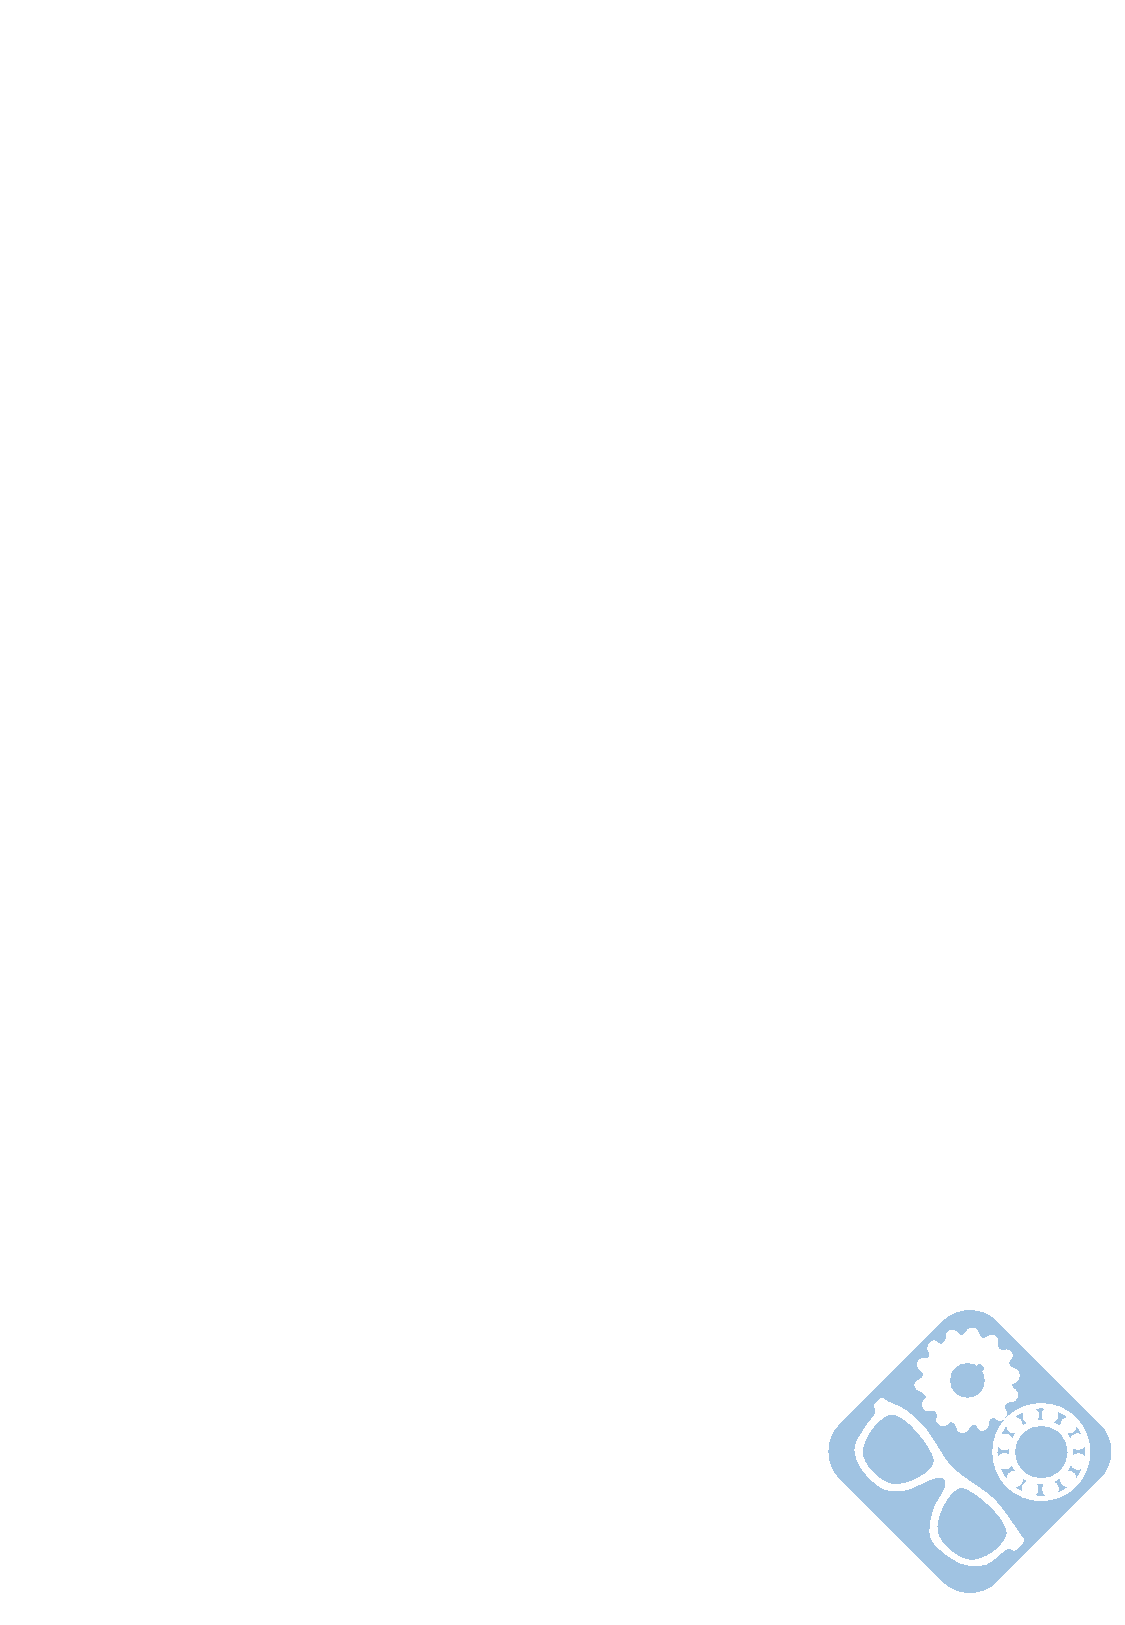
\includegraphics[width=\paperwidth,height=\paperheight,%
keepaspectratio]{../../img/fond4}%
\end{center}
\vfill
}}}

\begin{document}

\pagestyle{empty}

\AddToShipoutPicture*{\BackgroundPic}


\includegraphics[width=2cm]{../../img/logo}

\Huge{DS \num\ - \sujet}

\vspace{1cm}

\ifdef{\prive}{\begin{center}\colorbox{danger}{\Huge{Avec Correction}}\end{center}}{}

\begin{center}
\centering\huge{PTSI}
\end{center}

\vspace{2cm}


\begin{center}
\centering\Large{\jour}
\end{center}

\vspace{2cm}

\normalsize

\tableofcontents

\newpage

\AddToShipoutPicture{\BackgroundPicdeux}

\pagestyle{fancy}

\begin{center}
\Huge \sujet
\end{center}


\normalsize

\section{Présentation du support}

\subsection{Description du robot SPHERO}

Une nouvelle génération de robots à mobilité non conventionnelle a vu le jour avec la conception de robots en forme de sphère. Ces robots commencent à être utilisés dans des environnements difficiles (centrale nucléaire, terrain irrégulier) pour des missions d'inspection et de surveillance. Ce type de robot est aussi présent dans l'industrie du divertissement sous la forme d'objets connectés contrôlables avec un smartphone (ou tablette). C'est le cas du robot Sphero créé par la société Orbotix et qui sert de support d'étude pour ce sujet. 

Créé pour le loisir et l'éducation, le robot Sphero roule sur lui-même pour se déplacer. Une base robotique appelée module interne et dite différentielle (plateforme munie de deux roues motrices indépendantes, de même axe) est placée dans une sphère (le corps du robot) qui sert de liaison au sol et permet le déplacement (figure \ref{fig1}). Le Sphero est commandé par un smartphone avec lequel l'utilisateur guide le robot.

\begin{figure}[!ht]\begin{center}
 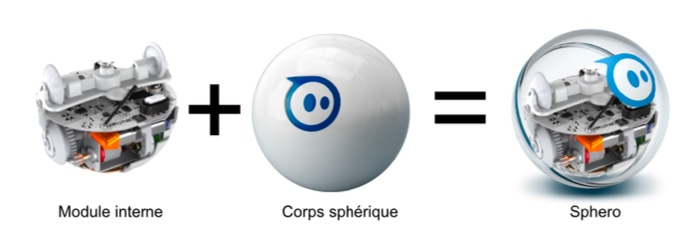
\includegraphics[width=0.8\linewidth]{img/figure_1}
 \caption{Constitution du SPHERO}
 \label{fig1}
\end{center}\end{figure}

Même si les consignes de l'utilisateur correspondent au comportement attendu du Sphero (cap et vitesse du corps sphérique), c'est en réalité le module interne que l'utilisateur commande grâce à son smartphone. Le principe de déplacement du Sphero peut être comparé à celui d'une roue de hamster : quand l'animal court à l'intérieur, il déplace le centre de gravité du système, ce qui fait tourner la roue. Ainsi, les deux roues motrices du module interne créent le roulement du corps sphérique du Sphero. 

\subsection{Manipulation et déplacement du robot SPHERO}

Pour commander le robot l'utilisateur dispose d'une application sur son smartphone (ou sa tablette). Une fois la connexion bluetooth établie entre le Sphero et le smartphone, l'utilisateur peut mettre en mouvement le robot grâce à une interface tactile (figure \ref{fig2}). L'utilisateur place son doigt au centre du cadran (sur le curseur ayant le sigle Sphero) puis le déplace dans le cadran. La position du doigt sur le cadran fournit une consigne de cap (par rapport à la marche avant) et de vitesse au robot : plus le doigt est éloigné du centre du cadran plus le robot va vite.

\begin{figure}[!ht]\begin{center}
 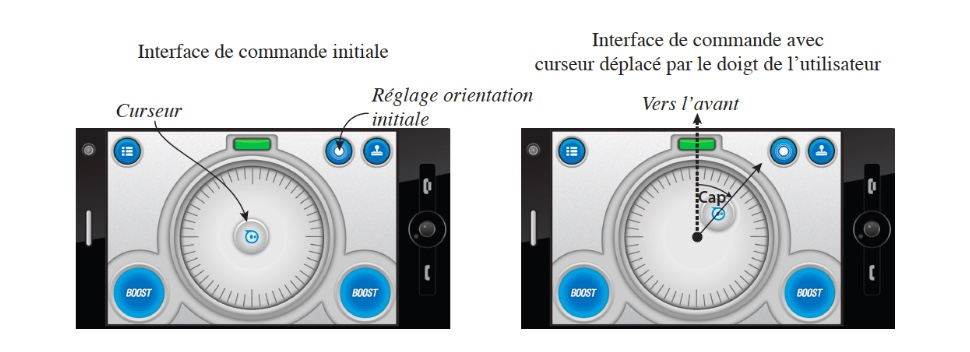
\includegraphics[width=0.8\linewidth]{img/figure_2}
 \caption{Interface Homme Machine (IHM) de commande du Sphero}
 \label{fig2}
\end{center}\end{figure}

\begin{figure}[!ht]\begin{center}
 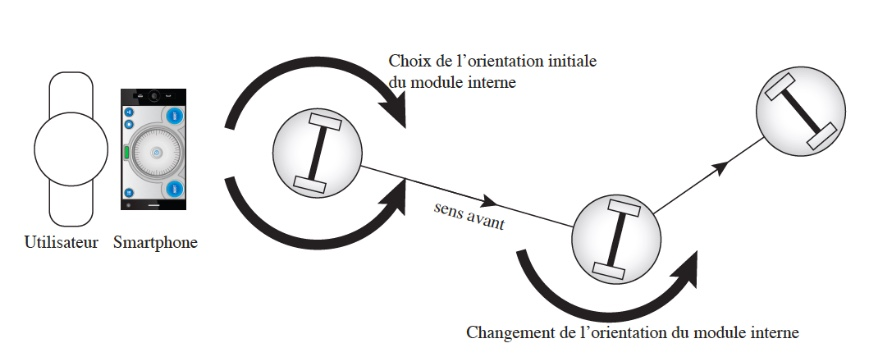
\includegraphics[width=0.8\linewidth]{img/figure_3}
 \caption{Déplacement du robot}
 \label{fig3}
\end{center}\end{figure}

\newpage

Un exemple de déplacement du robot Sphero est décrit par la figure \ref{fig3}. Pour un cap donné le Sphero se déplace selon une trajectoire rectiligne. Lorsque le cap est changé par l'utilisateur, le module interne change son orientation autour d'un axe vertical de lacet et une nouvelle direction est ainsi imposée au Sphero. Ce dernier reprend un déplacement en ligne droite suivant le nouveau cap. Afin que l'utilisation du robot soit à la hauteur des attentes de l'utilisateur, le robot Sphero doit satisfaire les exigences définies figure \ref{fig4}. 

\section{Étude préliminaire et respect de l'exigence 2 de maniabilité} 

Objectif : Évaluer les solutions techniques mises en jeu dans la conception du Sphero et déterminer une commande du Sphero permettant à ce robot d'atteindre les exigences de stabilité, de maniabilité et de respect des consignes de l'utilisateur. 
Un essai est réalisé avec le Sphero en mode non asservi. Les capteurs du robot ne sont pas utilisés pour la commande de ce dernier (figure \ref{fig5}). 

La figure \ref{fig5} montre la trajectoire suivie par le Sphero lors de l'essai. Le Sphero est en mode non asservi et connecté à un ordinateur (liaison sans fil). A l'écran de l'ordinateur est affiché un parcours délimité par deux lignes et l'utilisateur peut cliquer à l'écran pour imposer au Sphero une consigne de cap. Celle-ci correspond à la direction du vecteur ayant pour origine la position mesurée du Sphero au moment du clic et pour extrémité le point cliqué à l'écran. L'expérimentation est réalisée en intérieur et sans aucune perturbation pouvant altérer le fonctionnement du robot. La vitesse du robot est volontairement limitée à 50\% de sa vitesse maximale afin de rendre la manipulation plus aisée pour l'utilisateur. 


\begin{figure}[!ht]\begin{center}
 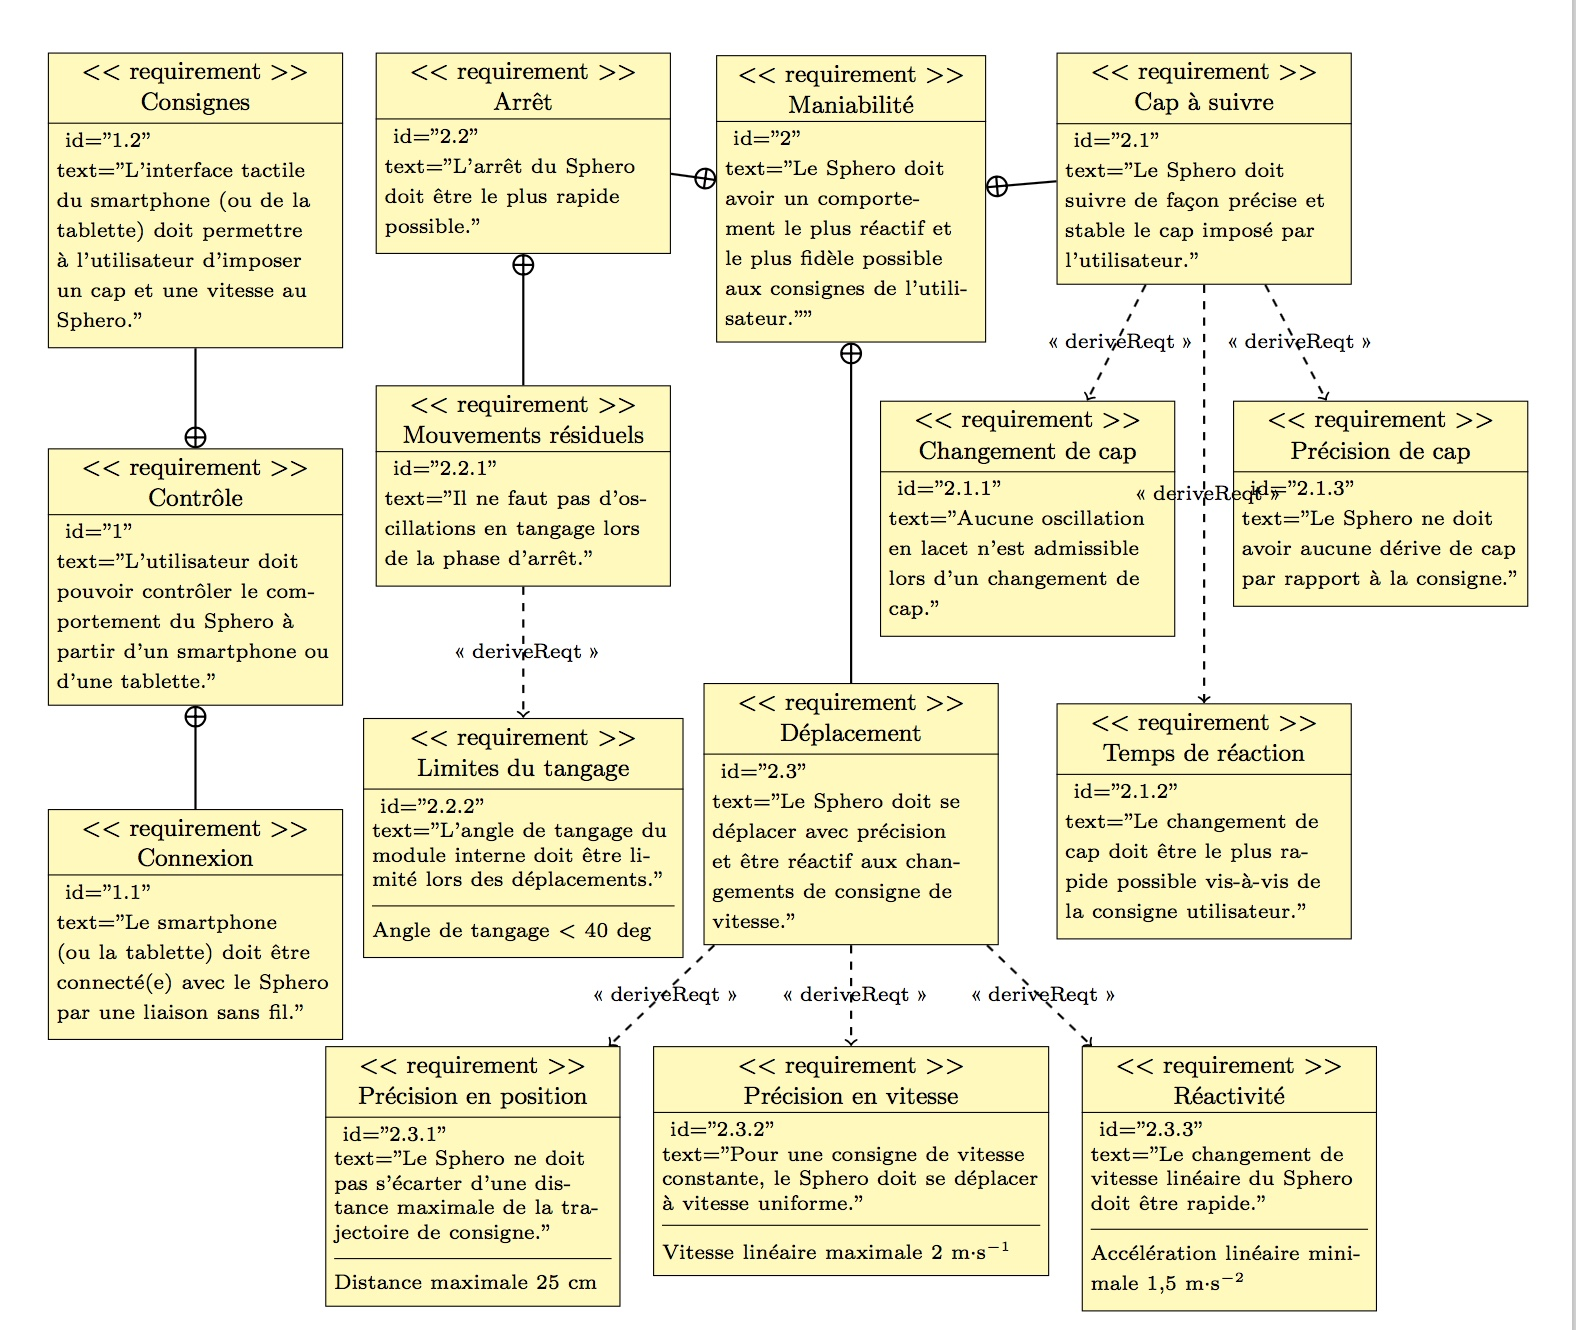
\includegraphics[width=\linewidth]{img/figure_4}
 \caption{Diagramme des exigences du SPHERO}
 \label{fig4}
\end{center}\end{figure}

\begin{figure}[!ht]\begin{center}
 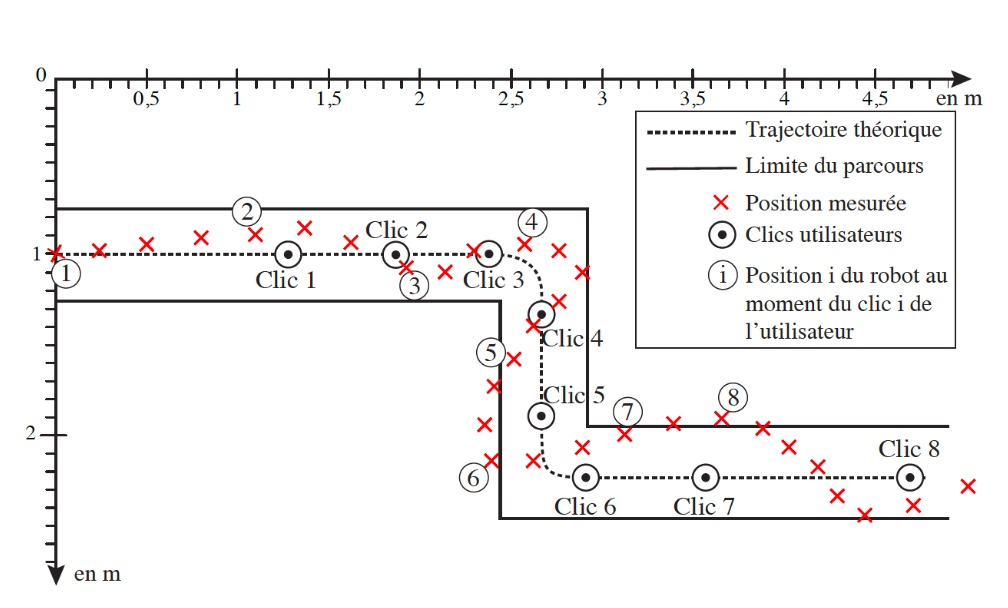
\includegraphics[width=\linewidth]{img/figure_5}
 \caption{Trajectoire du SPHERO}
 \label{fig5}
\end{center}\end{figure}

\question{En considérant le Sphero comme parfaitement asservi aux consignes de clic de l'utilisateur, quel serait le nombre minimal de consignes de changement de cap nécessaire pour faire évoluer le robot selon la trajectoire théorique ? Pour chacune de ces consignes de changement de cap quelle est la valeur du cap imposé (à l'instant initial, le cap est de 0 deg) ?}

\question{D'après l'expérimentation, l'exigence 2 de maniabilité est-elle respectée ? Justifier la réponse à partir du nombre d'actions de changement de cap réalisées par l'utilisateur lors de l'expérimentation.} 

~\

Au vu de l'essai analysé précédemment il apparait que sans commande spécifique le robot Sphero n'atteint pas toutes les exigences attendues. Le comportement précédemment observé impose à l'utilisateur de compenser sans cesse les défauts de trajectoire du Sphero, ce qui rend ce dernier difficilement maniable et donc inutilisable. 

La suite du sujet vise à résoudre ce problème. Deux aspects de la commande du robot Sphero seront étudiés : la génération des consignes de cap et de vitesse envoyées au Sphero et le principe de commande de la chaine d'énergie du Sphero. 

\section{Interfaçage utilisateur / Sphero (exigence 1 de contrôle)}
Une première approche de la commande du robot Sphero concerne la génération des consignes de cap et de vitesse à envoyer au robot.

Objectif : Concevoir un algorithme générant les consignes d'utilisation du Sphero (vitesse et cap) à partir de la manipulation de l'interface tactile. 

\subsection{Présentation de la technologie des écrans tactiles capacitifs}

Dans les écrans tactiles capacitifs simples, la surface de l'écran est recouverte d'une couche conductrice protégée par une couche isolante (verre, plastique, etc.). Lorsqu'un objet conducteur (comme le doigt de l'utilisateur) touche la couche isolante, il crée une capacité à l'endroit du contact. Etant donné que la couche conductrice est résistante, l'impédance mesurée à chaque coin de l'écran est différente et la comparaison des mesures effectuées aux quatre coins permet de localiser le point de contact. 

Les écrans tactiles capacitifs plus élaborés fonctionnent sur le même principe mais utilisent un réseau d'électrodes au lieu d'une couche conductrice continue, ce qui permet la détection de plusieurs points de contacts simultanés. Une unité de traitement récupère les mesures des capteurs et construit une matrice A, de mêmes dimensions que celles du réseau d'électrodes. La valeur d'un terme de A est d'autant plus élevée que l'électrode correspondante est plus proche d'un point de contact. 

\begin{figure}[!ht]\begin{center}
 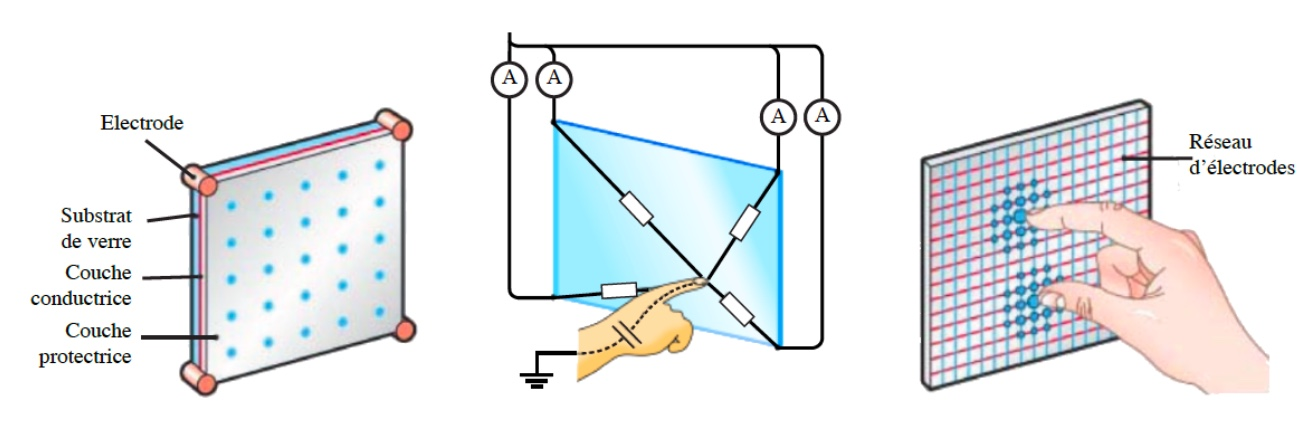
\includegraphics[width=0.8\linewidth]{img/figure_6}
 \caption{Écran tactile}
 \label{fig6}
\end{center}\end{figure}

\subsection{Interface graphique et respect de l'exigence 1}

La zone d'interface graphique utilisée pour guider le robot à partir d'un smartphone est présentée sur la figure \ref{fig7}. En faisant glisser le curseur à l'intérieur du cadran, l'utilisateur indique au SPHERO un consigne de cap et de vitesse.

\begin{figure}[!ht]\begin{center}
 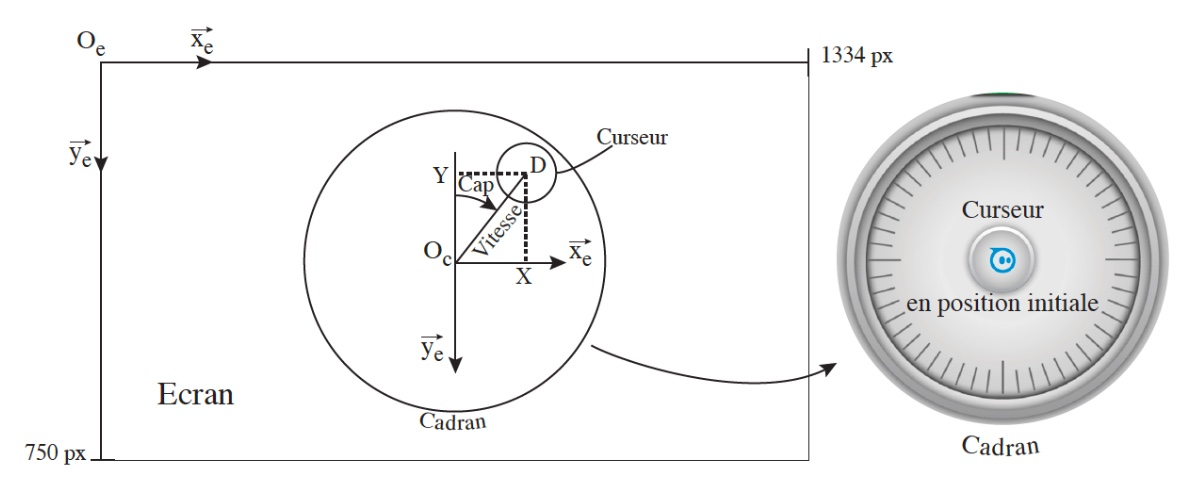
\includegraphics[width=0.8\linewidth]{img/figure_7}
 \caption{Paramétrage de l'interface tactile}
 \label{fig7}
\end{center}\end{figure}

L'écran considéré a une taille de 1334 × 750 pixels. On suppose que les pixels sont carrés et qu'à chaque pixel d'affichage est associé un point du réseau d'électrodes. 

\question{En déduire la largeur et la hauteur de l'écran en cm sachant que sa diagonale est de 4,7 pouces (11,938 cm).} 

\question{En déduire la taille en cm d'un pixel.}

\question{Calculer, en pixels, les dimensions de la surface de contact d'un doigt sachant qu'elle correspond approximativement à un carré d'une surface de $1\ cm^2$.}

\question{Le curseur circulaire de l'interface graphique est contenu dans un carré de largeur 170 pixels. Le choix du curseur est-il compatible avec le contrôle du Sphero par l'utilisateur ?} 

\newpage

Dans le programme Python de contrôle du Sphero à partir de l'interface tactile, la détection du doigt sur l'écran est gérée par trois fonctions :
\begin{itemize}
 \item \verb?Get_A()? renvoie la matrice A qui indique les points de contact sur l'écran tactile (voir section 3.1),
 \item \verb?On_cursor(A)? renvoie \verb?True? si le doigt de l'utilisateur est posé sur le curseur,
 \item  \verb?On_dial(A)? renvoie \verb?True? si le doigt de l'utilisateur est à l'intérieur du cadran.
\end{itemize}

\subsection{Consignes utilisateur}

Les consignes de cap à suivre et de vitesse sont élaborées à partir de la position du curseur (et donc du doigt) sur le cadran. La figure \ref{fig7} montre le repérage du curseur dans le cadran. Le repère $(O_e,\overrightarrow{x}_e,\overrightarrow{y}_e)$ est lié à l'écran (avec $O_e$ correspondant au bord supérieur gauche) et le point $O_c$ est au centre de l'écran et du cadran. A l'état initial le curseur se trouve au point $O_c$. La matrice A possède 750 lignes et 1334 colonnes. Le terme A[0][0] correspond géométriquement au point $O_e$ et les indices des termes de la matrice A correspondent aux coordonnées des pixels dans le repère $(O_e,\overrightarrow{x}_e,\overrightarrow{y}_e)$. 

Lors de la manipulation du curseur, son centre (noté D) est confondu avec le centre de la surface de contact du doigt avec l'écran. Ses coordonnées dans le repère $(O_c,\overrightarrow{x}_e,\overrightarrow{y}_e)$ sont notées $(X,Y)$. La fonction \verb?Get_XY(A)?, qui prend la matrice A en paramètre, renvoie un couple d'entiers correspondant aux coordonnées $(X,Y)$ de D, exprimées en pixels. 

\question{Donner l'expression de X et Y en fonction des indices du terme de la matrice A correspondant au point D.} 

~\

L'interface tactile permet de fournir les consignes de cap et de vitesse au Sphero. La consigne de cap est une consigne en degrés et celle de vitesse est une consigne en pourcentage (0\% pour l'arrêt et 100\% pour la vitesse maximale) qui correspond à l'éloignement du curseur par rapport au centre du cadran ; elle vaut 100\% quand $O_cD = 305$ pixels. Quant à la consigne de cap, elle est fournie par l'angle $(-\overrightarrow{y}_e,\overrightarrow{O_cD})$ exprimé en degrés dans l'intervalle [0, 360[. 

\question{Écrire en langage Python la fonction \verb?Get\_CV(X,Y)? qui prend en paramètre deux entiers correspondant à la position du curseur en pixels par rapport au centre du cadran et renvoie un couple de flottants \verb?(C,V)? correspondant aux consignes de cap et de vitesse correspondantes. Cette fonction renvoie \verb?(None, None)? si le point (X,Y) n'est pas à l'intérieur du cadran.}

~\

La fonction \verb?Set_heading(C)?, prenant pour argument C, transmet la consigne de cap C à la carte électronique du Sphero. Une seconde fonction \verb?Set_speed(V)?, prenant pour argument V , transmet la consigne de vitesse à la carte électronique du Sphero. 

\subsection{Architecture détaillée du robot Sphero}

Le cahier des charges de l'interface tactile impose le fonctionnement suivant pour la commande du Sphero : si le doigt de l'utilisateur est posé sur le curseur alors, tant que ce dernier est à l'intérieur du cadran, le Sphero doit avancer dans la direction et à la vitesse indiquée par la position du curseur dans le cadran. Dès que le doigt de l'utilisateur n'est plus en contact avec le curseur, le Sphero doit s'arrêter (le curseur retourne au centre du cadran). Le curseur accompagne toujours le doigt tant qu'il n'est pas levé. Si le curseur quitte le cadran, alors le Sphero poursuit sa route avec les dernières consignes de cap et de vitesse. L'utilisateur pourra reprendre le contrôle en replaçant le curseur dans le cadran. 

\question{Ecrire en Python l'algorithme de commande respectant le fonctionnement décrit précédemment et utilisant les fonctions données précédemment (qu'il n'est pas demandé d'écrire en Python). L'algorithme attendu a pour fonction d'expliciter la logique générale de commande du Sphero, il commencera ainsi:}

\begin{verbatim}
while True: # tant que le Sphero n'est pas éteint
    A = Get_A() 
    ... 
\end{verbatim}

La génération des consignes de cap et de vitesse ainsi que l'interfaçage support tactile/Sphero étant définis par l'étude menée précédemment, il convient de s'intéresser à l'architecture détaillée du robot et à ses performances. Ces dernières devant être en accord avec les exigences attendues, il est nécessaire d'évaluer les capacités du robot afin de déterminer la nécessité ou non d'une commande spécifique. 

\section{Architecture  détaillée du robot Sphero}

La composition du robot est fournie par le diagramme de définition des blocs figure \ref{fig8}. 

\begin{figure}[!ht]\begin{center}
 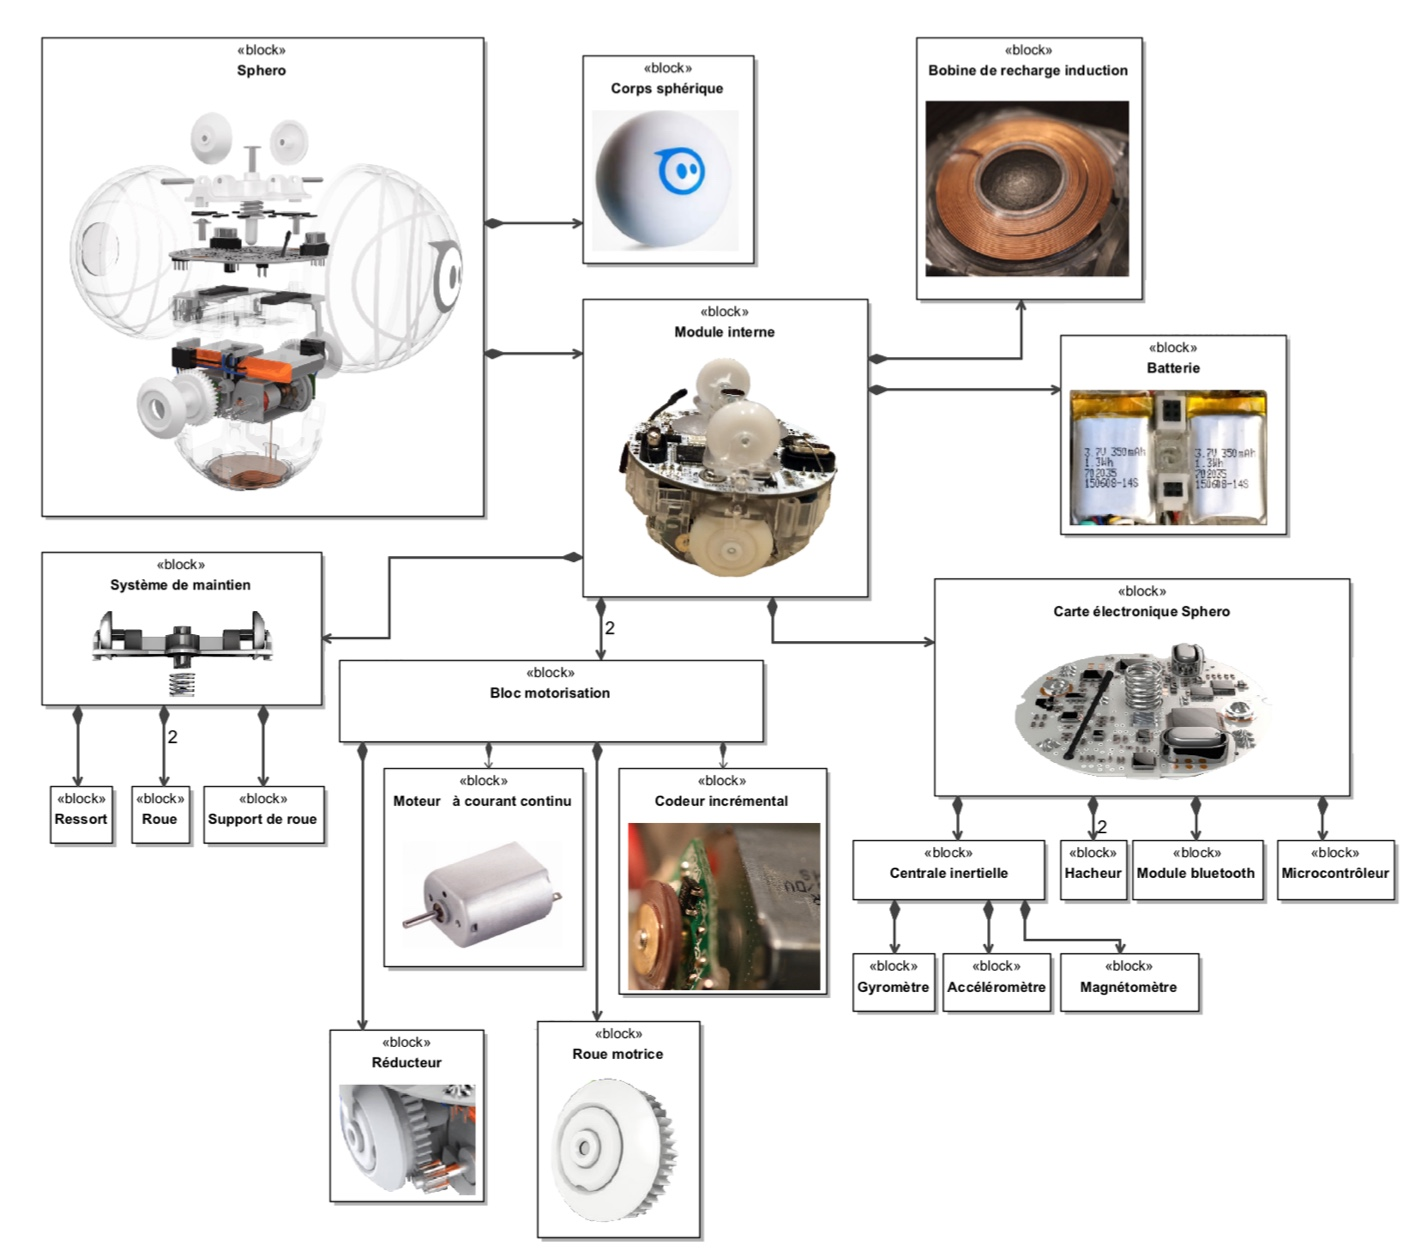
\includegraphics[width=0.85\linewidth]{img/figure_8}
 \caption{Diagramme de définition des blocs du Sphero}
 \label{fig8}
\end{center}\end{figure}

L'avance et l'orientation du robot sont créées par le module interne qui possède deux blocs de motorisation identiques et indépendants (comprenant chacun en particulier une roue motrice et un moteur). Le module interne est également équipé d'une centrale inertielle composée d'un magnétomètre (mesure du champ magnétique terrestre), d'un accéléromètre numérique (qui calcule les déplacements selon trois axes par double intégration des accélérations mesurées) ainsi que d'un gyromètre (mesure des vitesses de rotation en ($deg.s^{-1}$) autour de trois axes) permettant d'acquérir les informations décrites par la figure \ref{fig9}.

\question{Compléter sur la figure du document réponse la description chaîne d'information / chaîne d'énergie du robot Sphero.}

~\

La composition du robot est fournie par le diagramme de définition des blocs figure \ref{fig8}. 

\begin{figure}[!ht]\begin{center}
 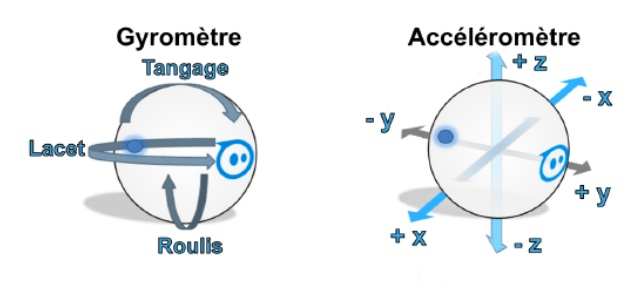
\includegraphics[width=0.5\linewidth]{img/figure_9}
 \caption{Illustration des informations acquises par la centrale inertielle}
 \label{fig9}
\end{center}\end{figure}

\vspace{-1.5cm}

\section{Déplacement et réglage de cap du robot Sphero} 

Le robot est équipé de deux actionneurs (moteurs électriques à courant continu) indépendants. Il est de fait nécessaire de mettre en évidence le lien entre le comportement du robot Sphero et celui des actionneurs. 

Objectif: Mettre en évidence la relation entre les actionneurs et le comportement du Sphero, afin de déterminer la façon dont les actionneurs doivent être commandés. 

\subsection{Modélisation et paramétrage}

\begin{figure}[!ht]\begin{center}
 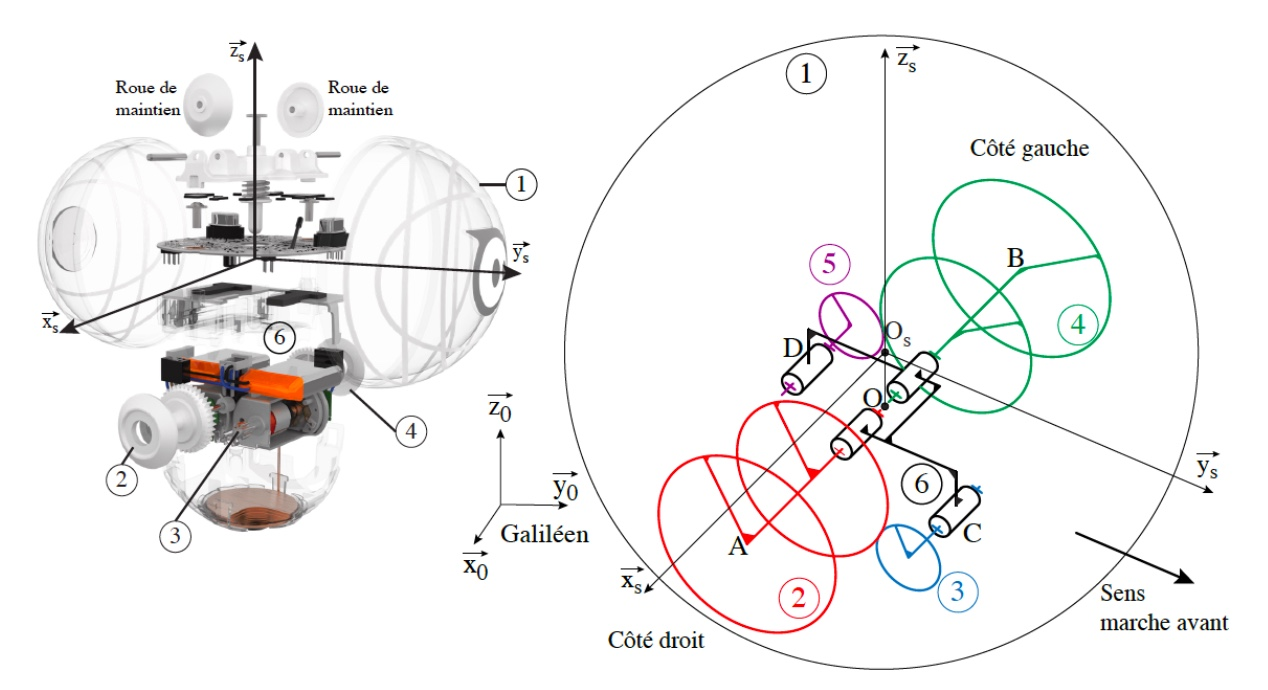
\includegraphics[width=0.67\linewidth]{img/figure_10}
 \caption{Schéma cinématique 3D du Sphero (sans le système de maintien)}
 \label{fig10}
\end{center}\end{figure}

1 désigne le corps sphérique du robot, 2 la roue motrice droite, 3 l'arbre moteur denté droit, 4 la roue motrice gauche, 5 l'arbre moteur denté gauche et 6 le châssis du module interne. Par la suite la désignation « module interne » correspond à l'ensemble 2+3+4+5+6. 

\begin{figure}[!ht]\begin{center}
 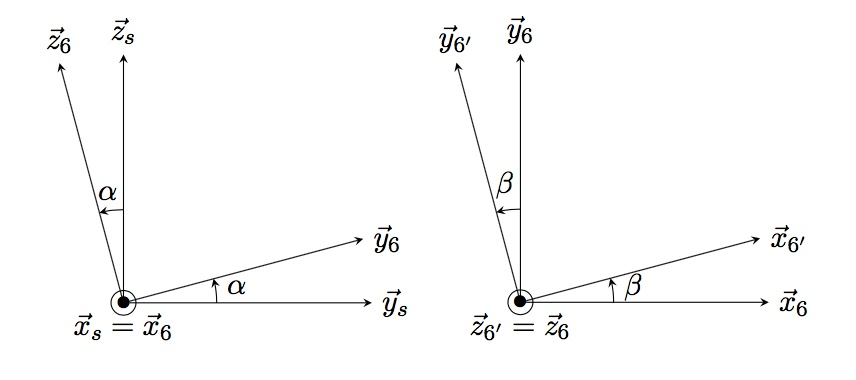
\includegraphics[width=0.6\linewidth]{img/figure_11}
 \caption{Définition des repères $R_G$ et $R_{G'}$}
 \label{fig11}
\end{center}\end{figure}

Le repère $R_S(O_S,\overrightarrow{x}_S,\overrightarrow{y}_S,\overrightarrow{z}_S)$ accompagne le robot Sphero et est tel que $\overrightarrow{z}_S=\overrightarrow{z}_0$ à chaque instant du mouvement, avec $\overrightarrow{z}_0$ la verticale du lieu et $\overrightarrow{y}_S$ dans la direction d'avance du robot. Le point $O_S$ correspond au centre du corps sphérique du robot.

Le châssis du module interne possède une mobilité en lacet et une en tangage par rapport au corps du Sphero. 
Le roulis du châssis du module interne par rapport au corps sphérique 1 n'est pas possible du fait de la forme des roues et de leur matière. 

Le repère $R_6(O,\overrightarrow{x}_6=\overrightarrow{x}_S,\overrightarrow{y}_6,\overrightarrow{z}_6)$ se déduit du repère $R_S$ par rotation d'angle $\alpha$ autour de l'axe $(O,\overrightarrow{x}_S)$. Cet angle $\alpha$ définit l'angle de tangage du châssis du module interne par rapport au repère $R_S$.

Le repère $R_{6'}(O,\overrightarrow{x}_{6'},\overrightarrow{y}_{6'},\overrightarrow{z}_{6'}=\overrightarrow{z}_6)$ lié au châssis du module interne, se déduit du repère $R_6$ par rotation d'angle $\beta$ autour de l'axe $(O,\overrightarrow{z}_6)$. Cet angle $\beta$ définit l'angle de lacet du châssis du module interne par rapport au repère $R_S$.

\begin{figure}[!ht]\begin{center}
 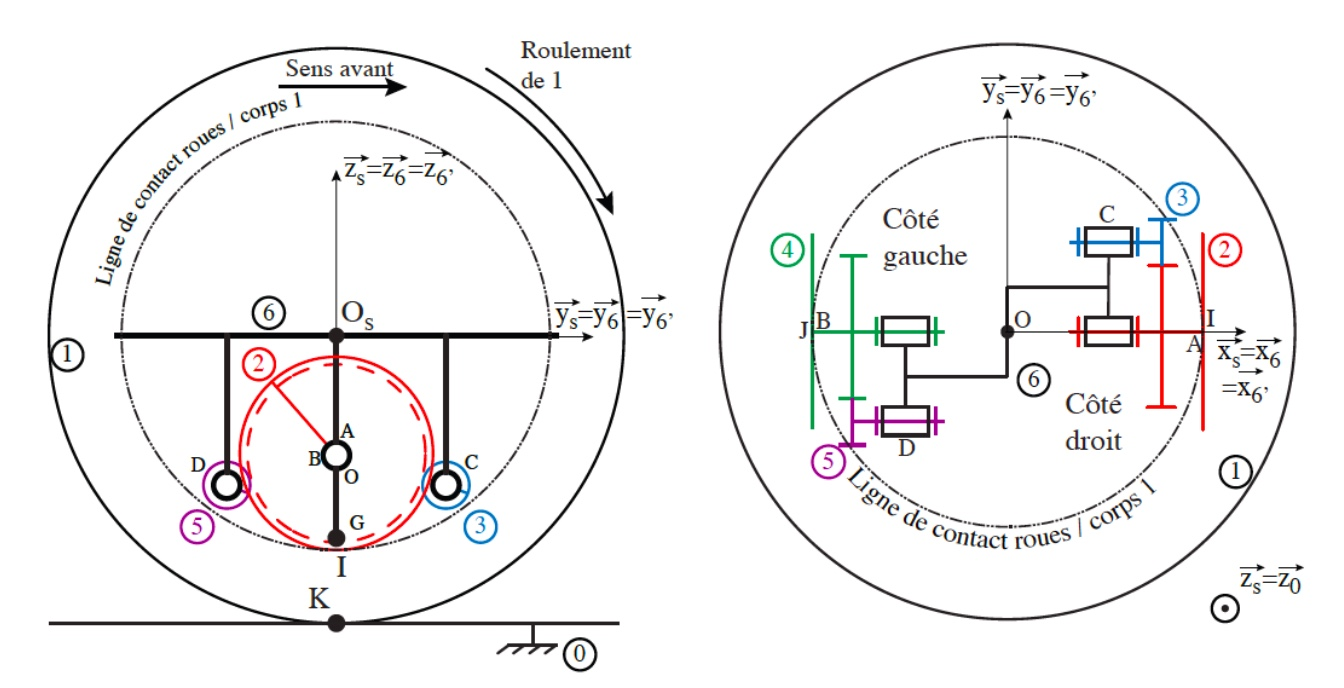
\includegraphics[width=0.85\linewidth]{img/figure_12}
 \caption{Schéma cinématique du Sphero pour $\alpha=0$ et $\beta=0$ (vue de côté et vue de dessus)}
 \label{fig12}
\end{center}\end{figure}

La figure \ref{fig12} propose un schéma cinématique du Sphero projeté dans le plan $(O,\overrightarrow{y}_S,\overrightarrow{z}_S)$ ainsi que dans le plan $(O,\overrightarrow{x}_S,\overrightarrow{y}_S)$ (le système de maintien n'est pas pris en compte). 

Le graphe des liaisons du robot Sphero (sans le système de maintien) est présenté figure \ref{fig13}.

\begin{figure}[!ht]\begin{center}
 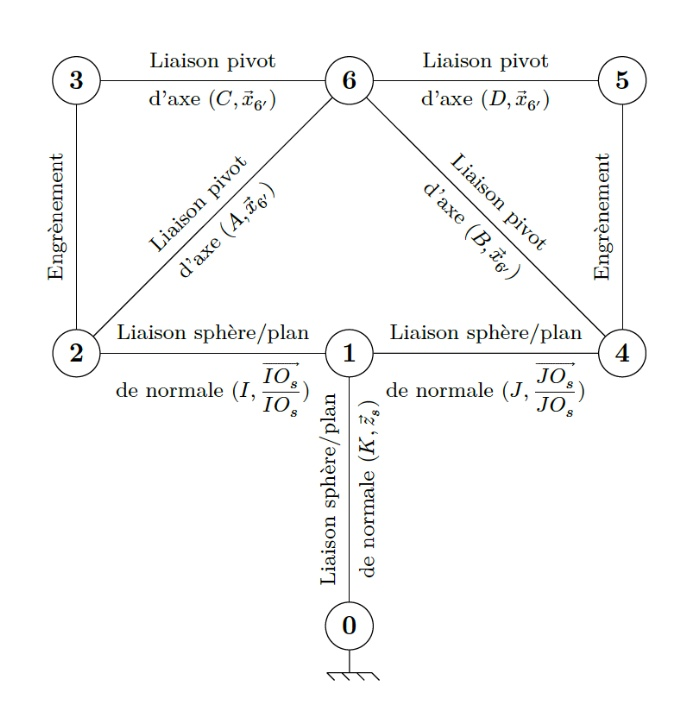
\includegraphics[width=0.6\linewidth]{img/figure_13}
 \caption{Graphe des liaisons du Sphero}
 \label{fig13}
\end{center}\end{figure}

Hypothèses:

L'hypothèse de roulement sans glissement sera adoptée au point I (point de contact 2/1), au point J (point de contact 4/1) et au point K (point de contact 1/0). 

~\

Modèles cinématiques:
\begin{itemize}
 \item les torseurs cinématiques sont notés: 

$\left\{V_{i/j}\right\}=\left\{
\begin{matrix}
 \omega_{xij} & {V_x }_{Mij} \\
 \omega_{yij} & {V_y }_{Mij} \\
 \omega_{zij} & {V_z}_{Mij} 
\end{matrix}
\right\}_{M,R_{6'}}=\left \{\begin{matrix} \vec {\omega _{i/ j}} \\ 
 \overrightarrow {V_{M,i/j}}\end{matrix}\right \}_M$,
 \item Le torseur cinématique de la liaison 2/1 s'écrit en I:
 
$\left\{V_{2/ 1}\right\}=\left\{
\begin{matrix}
 \omega_{x21} & {V_x }_{I21} \\
 \omega_{y21} & {V_y }_{I21} \\
 \omega_{z21} & {V_z}_{I21} 
\end{matrix}
\right\}_{I,R_{6'}}=\left \{\begin{matrix} \omega_{x21}.\vec{x}_{6'}+\omega_{y21}.\vec{y}_{6'}+\omega_{z21}.\vec{z}_{6'} \\ 
 {V_x }_{I21}.\vec{x}_{6'}+{V_y }_{I21}.\vec{y}_{6'}+{V_z}_{I21}.\vec{z}_{6'}\end{matrix}\right \}_{I}$
 \item Le torseur cinématique de la liaison 4/1 s'écrit en J:
 
$\left \{V_{4/ 1}\right\}=\left\{
\begin{matrix}
 \omega_{x41} & {V_x }_{J41} \\
 \omega_{y41} & {V_y }_{J41} \\
 \omega_{z41} & {V_z}_{J41} 
\end{matrix}
\right\}_{J,R_{6'}}=\left \{\begin{matrix} \omega_{x41}.\vec{x}_{6'}+\omega_{y41}.\vec{y}_{6'}+\omega_{z41}.\vec{z}_{6'} \\ 
 {V_x }_{J41}.\vec{x}_{6'}+{V_y }_{J41}.\vec{y}_{6'}+{V_z}_{J41}.\vec{z}_{6'}\end{matrix}\right \}_{J}$
 \item Le torseur cinématique $\left \{V_{6/ 1}\right\}$ en $O_S$ est de la forme:
 
$\left \{V_{6/ 1}\right\}=\left\{
\begin{matrix}
 \omega_{x61} & 0 \\
 0 & 0 \\
 \omega_{z61} & 0 
\end{matrix}
\right\}_{O_S,R_{6'}}=\left \{\begin{matrix} \omega_{x61}.\vec{x}_{6'}+\omega_{z61}.\vec{z}_{6'} \\ 
 \vec{0}\end{matrix}\right \}_{O_S}$
 \item $\omega_{x61}$ correspond à la vitesse angulaire en tangage du châssis du module interne par rapport au corps sphérique 1 du Sphero, et $\omega_{z61}$ correspond à la vitesse angulaire en lacet du châssis du module interne par rapport au corps sphérique 1 du Sphero.
 \item Les autres liaisons mécaniques ont aussi leur torseur cinématique défini dans le repère $R_{6'}$.
\end{itemize}


Données:
\begin{itemize}
 \item $\vec{IA}=R\vec{z}_{6'}=\vec{JB}$ avec $R=8mm$ rayon de la roue motrice 2,
 \item $\vec{OA}=L\vec{x}_{6'}=-\vec{OB}$,
 \item $\vec{O_SK}=-R_S\vec{z}_S$ avec $R_S=74mm$ rayon du corps sphérique 1,
 \item $\vec{OO_S}=h_r\vec{z}_{6'}$ avec $h_r=15mm$,
 \item le rapport de réduction entre 2 et 3 (et entre 4 et 5) est noté k avec 
 $k=0,21=\left|\frac{\omega_{26}}{\omega_{36}}\right|=\left|\frac{\omega_{46}}{\omega_{56}}\right|$
\end{itemize}

\question{En utilisant l’hypothèse de roulement sans glissement en I et en J, simplifier les expression de $\left \{V_{2/ 1}\right \}$ et $\left \{V_{4/ 1}\right\}$}

\question{En exploitant la fermeture cinématique 2-6-4-1 en J, montrer qu’il est possible d’écrire que $\omega_{z21}=k\frac{R}{2L}(\omega_{x36}-\omega_{x56})$ avec $\omega_{x36}$ la vitesse angulaire du moteur droit et $\omega_{x56}$ celle du moteur gauche.}

\question{Écrire la composition des vecteurs vitesse angulaire entre les pièces 1, 2 et 6. En déduire une relation entre $\omega_{z61}$, $\omega_{x61}$ et $\omega_{z21}$.}

\question{En déduire une relation de la forme $\omega_{z61}=\lambda(\omega_{x36}-\omega_{x56})$ avec $\lambda$ à déterminer.}

\question{Écrire une composition de vecteurs vitesses au point A entre les pièces 6, 1 et 2. En déduire une relation entre $\omega_{x21}$ et $\omega_{z61}$.}

\question{En déduire une relation de la forme $\omega_{x61}=\mu(\omega_{x36}+\omega_{x56})$ avec $\mu$ à déterminer.}

~\

Pour la suite, on prendra $\lambda=0,074$ et $\mu=0,105$.

Lors d’un changement de cap du Sphero le châssis du module interne admet un mouvement de lacet autour de l’axe $(O_S,\overrightarrow{z}_{6’})$. Le cap du robot Sphero est en fait imposé par celui du module interne. Le lacet du châssis du module interne ne doit pas induire de tangage car l’avance et le changement de cap du Sphero doivent être indépendants.
 
\subsection{Comportement des actionneurs pour un changement de cap}

\question{Quelle doit être la valeur de $\omega_{x61}$ lors d’un changement de cap?}

\question{En déduire la relation entre les vecteurs vitesse angulaire des moteurs du Sphero lors d’un changement de cap.}

\subsection{Comportement des actionneurs pour un déplacement en ligne droite}

\question{Quelle est la valeur de $\omega_{z61}$ lorsque le Sphero se déplace en ligne droite?}

\question{En déduire la relation entre les vecteurs vitesse angulaire des moteurs du Sphero afin que ce dernier puisse se déplacer en ligne droite.}

\subsection{Vitesse d’avance et respect de l’exigence 2.3 de déplacement}

Au point K de contact entre le corps 1 et le sol noté 0, il y a roulement sans glissement et donc le torseur cinématique de la liaison 1/0 s’écrit en K:
$\left \{V_{1/ 0}\right \}=
\left \{\begin{matrix} \omega_{x10}.\vec{x}_S+\omega_{y10}.\vec{y}_S+\omega_{z10}.\vec{z}_S \\ 
 \vec{0}\end{matrix}\right \}_{K}$
 
\question{Lors d’un mouvement d’avance en ligne droite, donner la relation entre $\omega_{x10}$, $R_S$ et $v$ la vitesse d’avance du robot par rapport au sol $(v=\vec{V}_{O_S\in1/0}.\vec{y}_S)$}

Pour cette étude, on se place en régime établi où l’angle de tangage $\alpha$ du module interne est constant. 

\question{Pour $\alpha$ constant et toujours lors d’un déplacement en ligne droite $(\vec{x}_S=\vec{x}_6=\vec{x}_{6’})$, que vaut la composante $\omega_{x60}=\vec{\Omega}_{6/0}.\vec{x}_S$ correspondant à la vitesse de tangage du module interne par rapport au sol?}

\question{En déduire la relation entre $\omega_{x10}$ et $\omega_{x61}$.}

Le constructeur du robot Sphero annonce une vitesse maximale d’avance en ligne droite $v=\vec{V}_{O_S\in1/0}.\vec{y}_S= 2 m.s^{-1}$ alors que les moteurs possèdent une vitesse angulaire maximale de $1200 tr.min^{-1}$.

\question{Déterminer l’expression de v en fonction de $\omega_{x36}$ et $\omega_{x56}$. Faire l’application numérique et conclure sur le respect de l’exigence 2.3}

\section{Performances en changement de cap du Sphero (exigence 2.1 de suivi de cap}

Objectif: déterminer la loi de commande en lacet du mode interne qui permettra le respect des exigences de cap lors de l’utilisation du Sphero (exigences 2.1, 2.1.1 et 2.1.2).

Lors d’un réglage de cap le module interne admet un mouvement de lacet d’angle $\beta$ (voir figure \ref{fig14}). Le cap du robot Sphero est imposé par celui du module interne. 

\begin{figure}[!ht]\begin{center}
 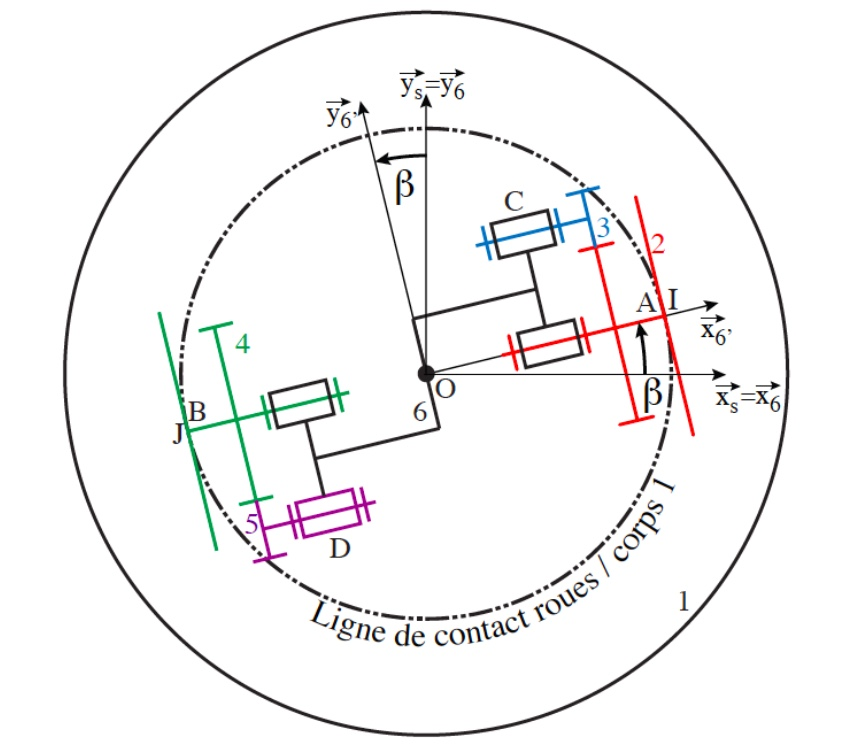
\includegraphics[width=0.55\linewidth]{img/figure_14}
 \caption{ Schéma cinématique plan du Sphero en vue de dessus avec $\alpha=0$ et $\beta\neq0$}
 \label{fig14}
\end{center}\end{figure}

Lors de la rotation du module interne autour de l’axe $(O,\overrightarrow{z}_{6’})$ aucun mouvement de lacet du corps sphérique 1 n’est induit. Ceci est rendu possible du fait de l’action combinée des deux moteurs associée à la résistance au roulement au niveau du contact Sphero/sol.

L’étude proposée dans cette partie est réalisée robot à l’arrêt. Si les performances en lacet du module sont satisfaisantes dans ces conditions, elles le seront également en mouvement car le fait que le robot avance n’induit pas de perturbations sur le lacet du module interne.

Lors du réglage de cap, le mouvement du module interne est un mouvement de rotation autour de l’axe $(O,\overrightarrow{z}_{6’})$,le corps 1 étant considéré immobile $\overrightarrow{z}_{6’}=\overrightarrow{z}_6 $.

Les moteurs devant avoir la même vitesse angulaire, la notation suivante est adoptée : $\omega_{x36}=\omega_m(t)=\omega_{x56}$.

Afin que les exigences 2.1, 2.1.1 et 2.1.2 soient vérifiées par le robot, les performances données tableau 2 doivent être atteintes. 


\begin{table}[!h]
\begin{tabular}{|c|c|c|}
\hline
Performance & Critère & Niveau \\
\hline
Précision angulaire & Erreur en position en régime permanent & Nulle pour une entrée en échelon \\
\hline
Rapidité & Temps de réponse à 5\% & $t_{r5\%}\leq 0,3s$ \\
\hline
Stabilité & Dépassement & aucun \\
\hline
\end{tabular}
\caption{Exigences du système}
\label{tab1}
\end{table}

La loi entrée-sortie de la transmission mécanique étant connue, l’objectif est maintenant d’évaluer les performances de la commande en lacet du module interne. Dans un premier temps la commande étudiée sera sans correction afin de mettre en évidence les performances intrinsèques liées au choix de l’architecture de commande. La commande en lacet du module interne est décrite figure \ref{fig15}. 

La commande des motorisations se fait directement par l’acquisition de la vitesse de tangage $\omega_{z61}(t)$ du module interne et par une tension de consigne $u_C(t)$. Cette tension $u_C(t)$ est générée par un correcteur à partir de la différence entre l’orientation de consigne $\beta_C(t)$ du module interne et son orientation réelle $\beta(t)$ (information fournie par la centrale inertielle).

\begin{figure}[!ht]\begin{center}
 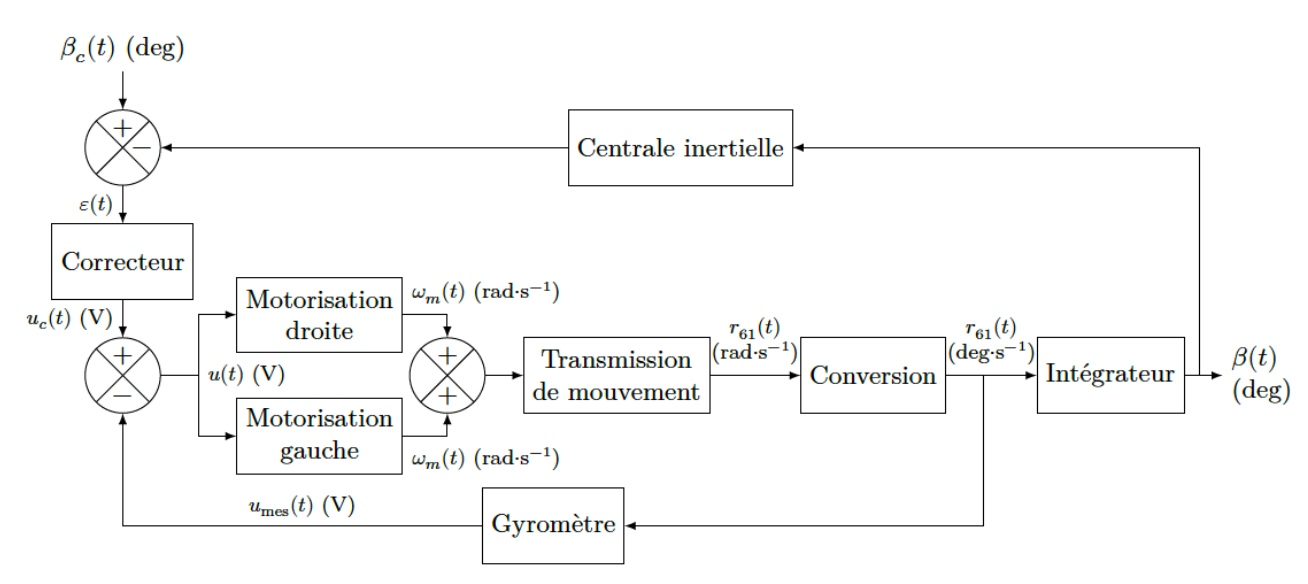
\includegraphics[width=\linewidth]{img/figure_15}
 \caption{Schéma fonctionnel de l’asservissement en lacet}
 \label{fig15}
\end{center}\end{figure}

\newpage

Données:
\begin{itemize}
 \item la centrale inertielle est modélisée par un gain unité;
 \item la fonction de transfert du correcteur est noté $C(p)$;
 \item la sensibilité du gyromètre est de $K_g=0,028V.s.deg^{-1}$;
 \item les blocs motorisation ont la même fonction de transfert $H_m(p)=\frac{\Omega_m(p)}{U(p)}=\frac{K_m}{1+\tau_m.p}$. Le bloc motorisation modélise l’ensemble hacheur+moteur: $-\omega_{z61}=2\lambda\omega_m(t)$.
\end{itemize}

\begin{figure}[!ht]\begin{center}
 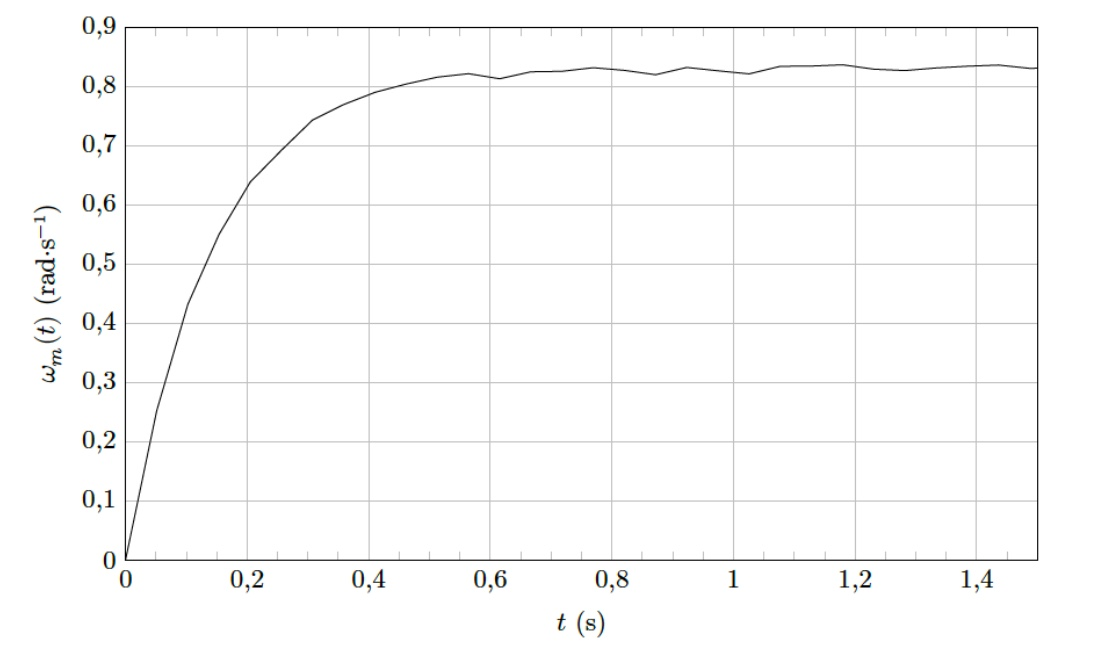
\includegraphics[width=0.8\linewidth]{img/figure_16}
 \caption{Réponse indicielle du moteur droit}
 \label{fig16}
\end{center}\end{figure}

La figure \ref{fig16} représente la réponse indicielle du moteur droit pour un essai avec un échelon d’entrée u(t)=1V. (Le bloc gauche donne la même réponse à la même sollicitation en entrée).

\question{En se plaçant dans le domaine de Laplace, compléter sur la figure du document réponse le schéma bloc de l’asservissement de l’angle de lacet du module interne.}

~\

Dans cette première étude de la commande, il n’y a pas de correction: $C(p)=1$.

\question{Déterminer l’expression sous forme canonique de la fonction de transfert en boucle fermée $H(p)=\frac{\beta(p)}{\beta_c(p)}$}

Pour la suite, la forme numérique de $H(p)$ est $H(p)=\frac{1}{ap^2+bp+1}$ avec $a=0,019s^2$ et $b=0,17s$.

\question{En utilisant l’abaque de la figure \ref{fig17} fournissant la valeur de $t_{r5\%}$ en fonction de $\xi$, déterminer le temps de réponse à $5\%$ du système de commande en lacet.}

\question{D’après les questions précédemment traitées, les performances requises pour l’asservissement sont-elles atteintes ? Justifier les réponses apportées.}

~\

Il apparaît que certaines performances de la commande en lacet sans correction sont à améliorer. L’utilisation d’un correcteur est nécessaire à l’optimisation du comportement en lacet précédemment mis en évidence.

\begin{figure}[!ht]\begin{center}
 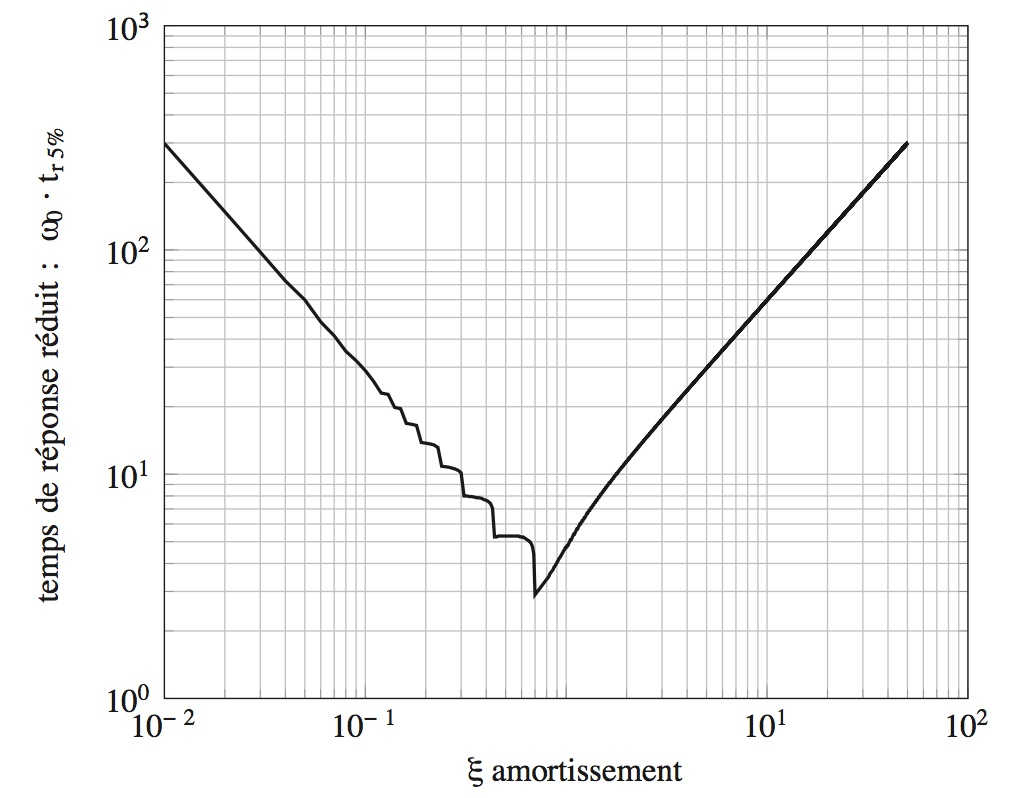
\includegraphics[width=0.7\linewidth]{img/figure_17}
 \caption{Abaque $\omega_0.t_{r5\%}=f(\xi)$}
 \label{fig17}
\end{center}\end{figure}

\newpage

\subsection{Optimisation de la commande de lacet}

La figure \ref{fig18} représente le comportement en lacet du module interne pour un essai indiciel $\beta_c=10\ deg$. Cet essai a été réalisé avec un correcteur à avance de phase (programme de PT) de la forme $C(p)=K_c\frac{1+bp}{1+ap}$ avec $a=0,01s$ et $b=0,12s$.

\begin{figure}[!ht]\begin{center}
 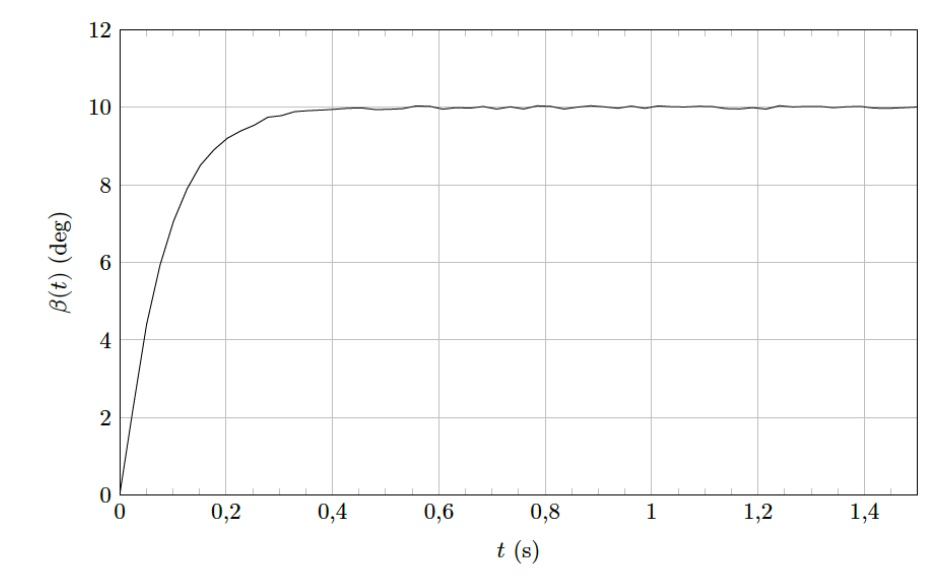
\includegraphics[width=0.7\linewidth]{img/figure_18}
 \caption{Réponse temporelle de la commande corrigée du Sphero}
 \label{fig18}
\end{center}\end{figure}

\question{Conclure sur les performances du système de commande en lacet du module interne une fois la correction appliquée.}

\newpage

\section{Étude de spécifications}

\begin{figure}[!ht]\begin{center}
 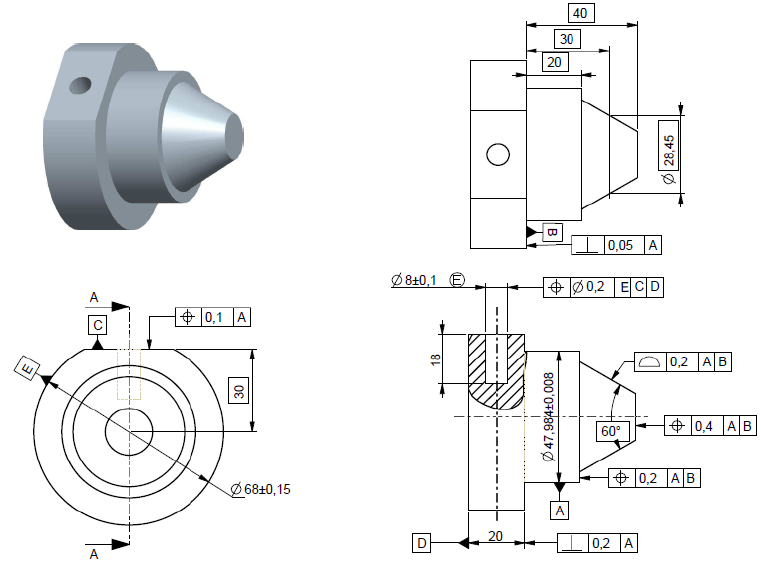
\includegraphics[width=\linewidth]{img/specifications}
 \caption{Dessin de définition}
 \label{fig19}
\end{center}\end{figure}

\question{Expliciter la spécification dimensionnelle 
\includegraphics[width=0.1\linewidth]{img/specif0}.}

\question{Décrire les spécifications géométriques suivantes.}

\begin{center}
 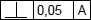
\includegraphics[width=0.2\linewidth]{img/specif1} \hspace{2cm} 
\includegraphics[width=0.2\linewidth]{img/specif2}
\end{center}

\section{Montage de roulements}

Nous proposons dans cette partie de concevoir un montage de roulements sur le montage de la figure \ref{fig20}.

\begin{figure}[!ht]\begin{center}
 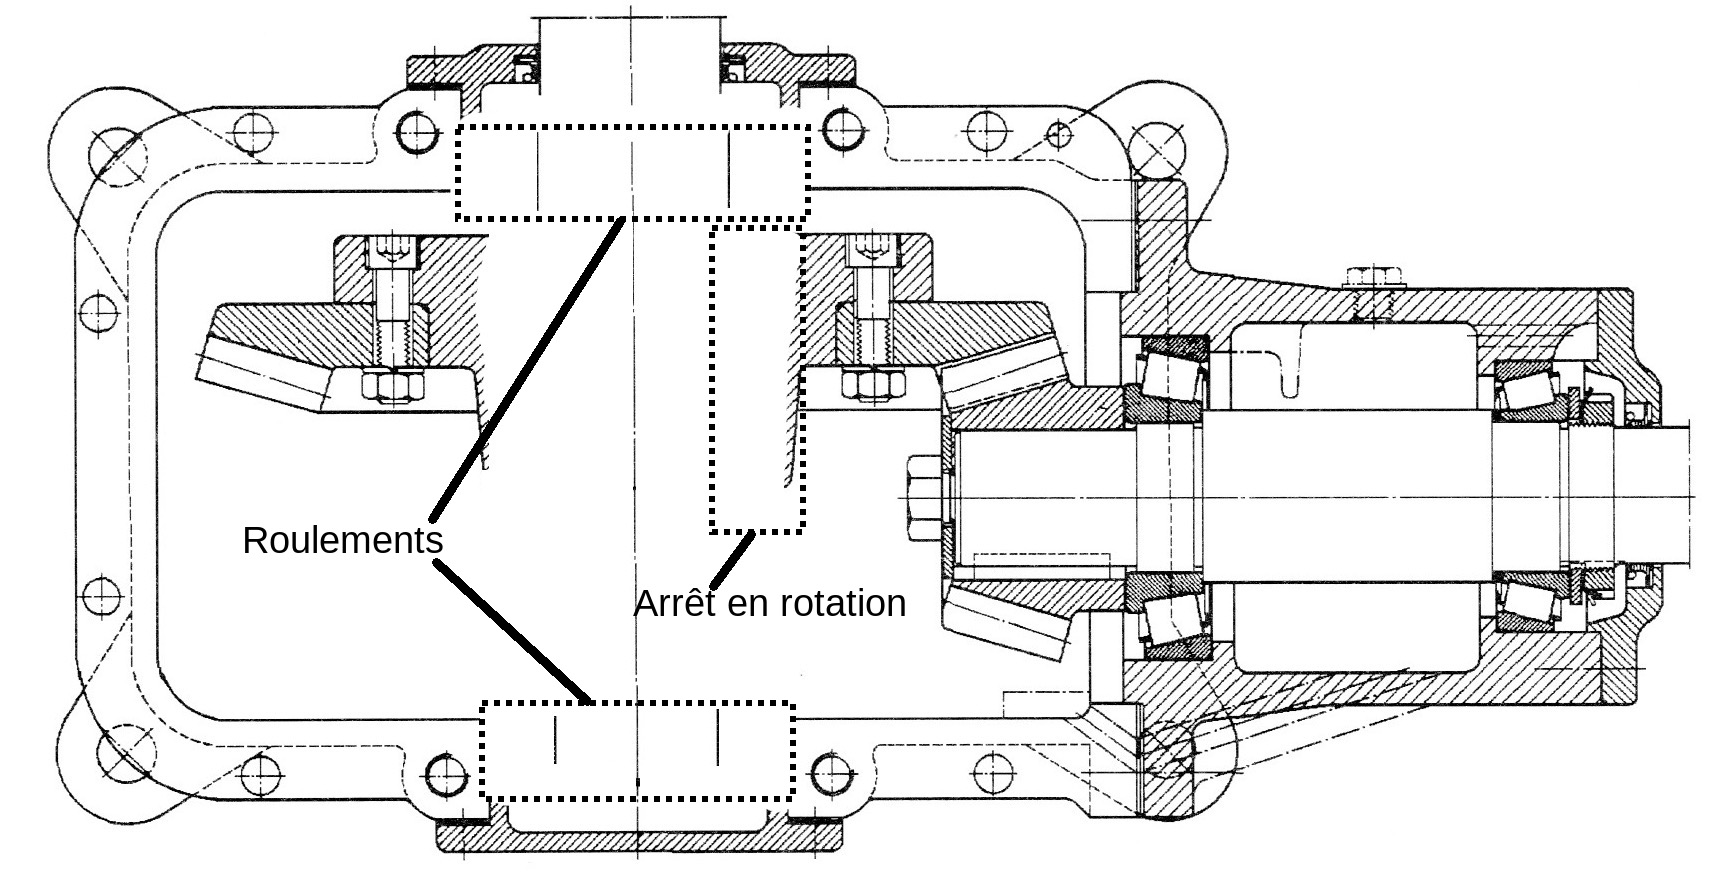
\includegraphics[width=\linewidth]{img/montage_roulements_sujet}
 \caption{Boîte de transmission}
 \label{fig20}
\end{center}\end{figure}

\question{Donner le plus d'informations possibles sur le montage présent à droite sur la figure \ref{fig19}, justifier ces choix.}

Le montage de roulement de gauche a été effacé, il est constitué de roulements à rouleaux coniques de même type que ceux du montage de droite. On remarquera que le carter dans lequel s'installe ces roulements n'est pas hachuré (contrairement à celui de droite).

\question{Expliquer pourquoi le carter n'est pas hachuré.}

\question{Proposer et justifier un montage de roulements pour cette zone.}

~\ \\

Dans la suite, il est demandé de concevoir l'assemblage de la liaison pivot effacée. Il faudra donc:
\begin{itemize}
 \item Mettre en place les roulements au niveau des cadres en pointillés (la position de l'arbre est présente sur le dessin),
 \item Mettre en place les arrêts axiaux en fonction du montage choisi à la question précédente et ainsi terminer la représentation des autres pièces,
 \item Montrer comment le réglage du jeu sera effectué,
 \item Mettre en place une solution par obstacle pour arrêter la rotation entre l'arbre et le pignon dans le cadre \og Arrêt en rotation \fg,
 \item Mettre en place les ajustements correspondants.
\end{itemize}

\question{Mettre en place les roulements et compléter le dessin des pièces environnantes. Montrer que le réglage du jeu dans le roulement est prévu.}

\question{Concevoir l'arrêt en rotation.}

\question{Mettre en place les ajustements nécessaires.}

\begin{center}
\Huge{FIN DE L'ENONCE}
\end{center}

\cleardoublepage

\pagestyle{documentreponse}

\section{Documents réponse}

\reponse{13}{}{Nombre minimal de consignes: 3. \\
Le trajet comporte 3 lignes droites et 2 virages. \\
Cap 0° à l'instant initial \\
Cap -90° pour le premier virage \\
Cap +90° pour le 2ème virage}

\reponse{13}{}{Le Sphero n’a pas une trajectoire précise:
\begin{itemize}
 \item oscillation de 0,8m à 1,2m pour la première ligne droite
 \item de 2,4m à 2,9m pour la seconde ligne droite
 \item de 1,5m à 2,6m pour la troisième ligne droite
\end{itemize}
Il ne respecte pas l’exigence 2.\\
Il y a 8 clip utilisateurs, et de gros écarts (notamment entre les clics 6 et 8).\\
2.3.1: la distance doit être inférieure à 25cm: non validée.\\
2.1.1: aucune oscillation en lacet: non validée.\\
2.1.3: aucune dérive de cap: non validée.}

\reponse{13}{}{Diagonale de 4,7 pouces soit 11,938 cm.
Astuce: en construisant un triangle rectangle, on peut approximer la largeur et la longueur de l’écran (on prend un triangle rectangle de 7,5cm par 13,34cm, pour garder les proportions des pixels de l’écran et on mesure la diagonale, qui fait environ 15,3 cm, correspondant à 15300 pixels et à la diagonale de 12cm dans la réalité. En prenant la bonne échelle, on trouve le résultat). \\
On obtient environ (6cm * 10,5cm)}

\reponse{7}{}{Si 750 pixels représentent 6cm alors 1 pixel mesure $\frac{6}{750}$
 cm de largeur soit environ $8.10^{-3}$ cm (selon les candidats, les approximations vont varier, l’important est de garder une démarche cohérente par rapport à la question 3)}

\reponse{11}{}{Si 750 pixels représentent 6cm alors 1 cm représente $\frac{750}{6}$ cm soit 125 pixels.\\
$1cm²$ contient alors 125.125 pixels soit 15625 pixels}

\reponse{11}{}{Curseur circulaire contenu dans un carré de 170 pixels de largeur, soit $170.8.10^{-3}$ cm
La zone est alors de  
La surface du doigt est de  
Le curseur circulaire étant contenu dans une surface supérieure à celle du doigt, le choix du curseur est compatible avec le contrôle du Sphero par l’utilisateur
}

\reponse{11}{}{Expression de X et Y en fonction des indices du terme de la matrice A correspondant au point D.\\
$X=X_D-667$,$Y=Y_D-375$}


\begin{SaveVerbatim}{VerbEnv}
import math as m
def Get_CV(X,Y) :
   if m.sqrt(X**2+Y**2)>305 :
      return (None,None)
   else :
      V=m.sqrt(X**2+Y**2)*100/305
      if Y<0 :
        C=m.acos(X/V)*180/m.pi
      else :
        C=(2*m.pi-m.acos(X/V))*180/m.pi
        return (C,V)
\end{SaveVerbatim}

\reponse{21}{}{\BUseVerbatim{VerbEnv}}

\begin{SaveVerbatim}{VerbEnv}
while True: # tant que le Sphero n'est pas éteint A = Get_A()
while On_Cursor(A)==True : 
     while On_dial(A)==True :
       (X,Y)=Get_XY(A)
       (C,V)=Get_CV(X,Y)
       Set_heading(c)
       Set_speed(V)
       A=Get_A()
     A=Get_A()
  Set_speed(0)
\end{SaveVerbatim}
\reponse{21}{}{\BUseVerbatim{VerbEnv}}

\newpage

\reponse{1}{\begin{center}
\includegraphics[width=\linewidth,angle=90]{img/DR1}\end{center}}{\begin{center}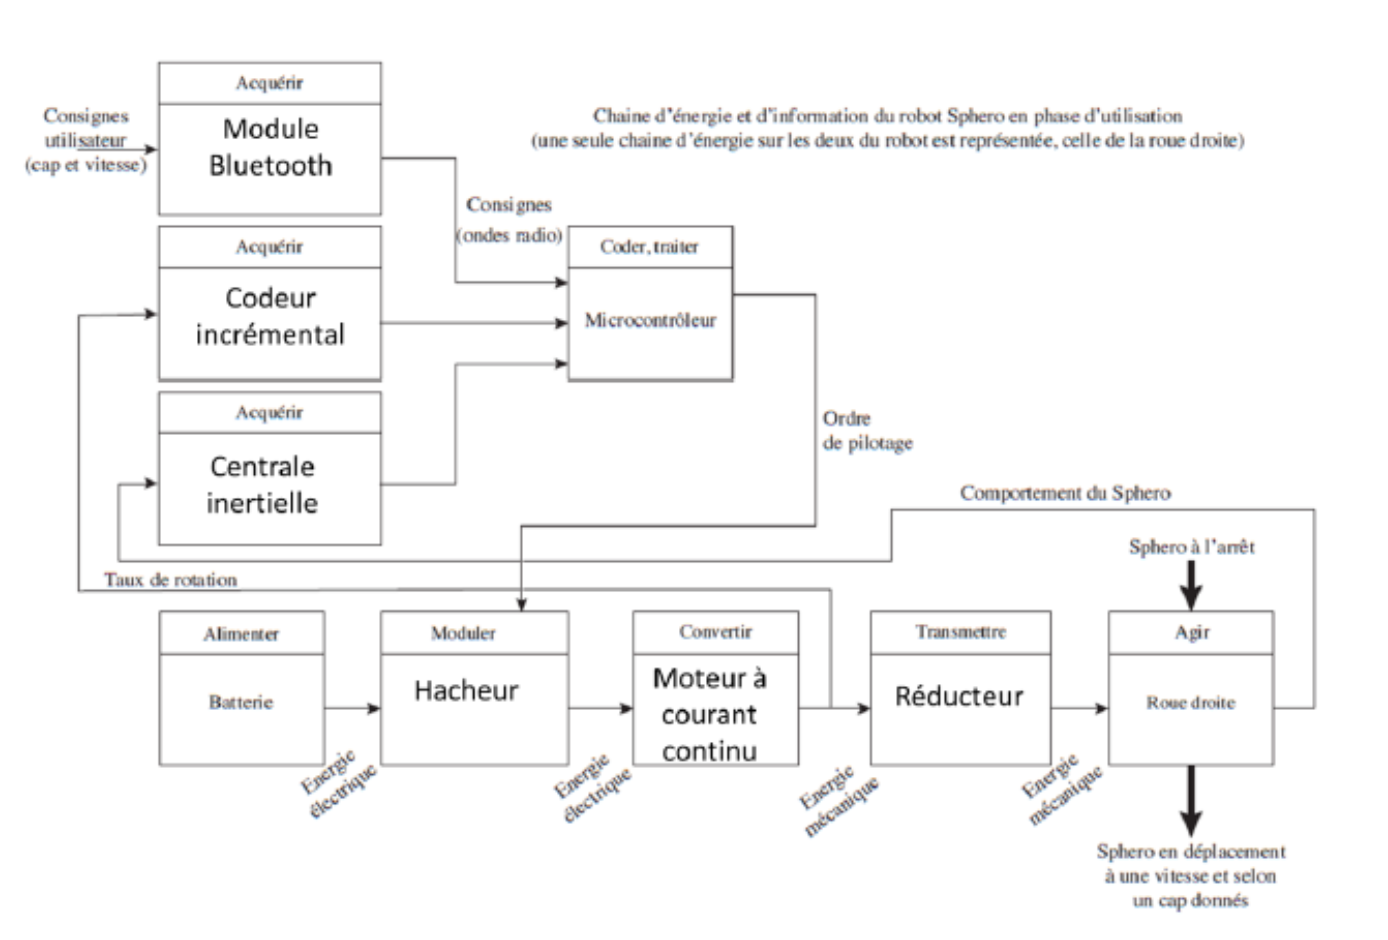
\includegraphics[width=\linewidth]{img/DR1_cor}\end{center}}

\newpage

\reponse{2}{$\left\{V_{2/1}\right\}=$\\ \vspace{2cm} \\ $\left\{V_{4/1}\right\}=$ \vspace{2cm}}{Hypothèse roulement sans glissement en I et J\\
$\left \{V_{2/ 1}\right \}=\left \{\begin{matrix} \vec{\Omega_{21}} \\ 
 \vec{0}\end{matrix}\right \}_{I} =
\left \{\begin{matrix} \omega_{x21}.\vec{x}_{6'}+\omega_{y21}.\vec{y}_{6'}+\omega_{z21}.\vec{z}_{6'} \\ 
 \vec{0}\end{matrix}\right \}_{I}$ \\
$\left \{V_{4/ 1}\right \}=\left \{\begin{matrix} \vec{\Omega_{21}} \\ 
 \vec{0}\end{matrix}\right \}_{J}=
\left \{\begin{matrix} \omega_{x41}.\vec{x}_{6'}+\omega_{y41}.\vec{y}_{6'}+\omega_{z41}.\vec{z}_{6'} \\ 
 \vec{0}\end{matrix}\right \}_{J}$}

\reponse{60}{}{$\left \{V_{4/ 1}\right \}=\left \{V_{4/ 6}\right \}+\left \{V_{6/ 2}\right \}+\left \{V_{2/ 1}\right \}$\\
$\left \{V_{4/ 1}\right \}=
\left \{\begin{matrix} \omega_{x41}.\vec{x}_{6'}+\omega_{y41}.\vec{y}_{6'}+\omega_{z41}.\vec{z}_{6'} \\ 
 \vec{0}\end{matrix}\right \}_{J}$\\
$\left \{V_{4/6}\right \}=
\left \{\begin{matrix} \omega_{x46}.\vec{x}_{6'} \\ 
 \vec{0}\end{matrix}\right \}_{B}=\left \{\begin{matrix} \omega_{x46}.\vec{x}_{6'} \\ 
 \overrightarrow{JB}\wedge\omega_{x46}.\vec{x}_{6'}\end{matrix}\right \}_{J}=\left \{\begin{matrix} \omega_{x46}.\vec{x}_{6'} \\ 
 R\omega_{x46}.\vec{y}_{6'}\end{matrix}\right \}_{J}$\\
$\left \{V_{6/2}\right \}=\left \{\begin{matrix} \omega_{x62}.\vec{x}_{6'} \\ 
 \vec{0}\end{matrix}\right \}_{A}=\left \{\begin{matrix} \omega_{x62}.\vec{x}_{6'} \\ 
 \overrightarrow{JA}\wedge\omega_{x62}.\vec{x}_{6'}\end{matrix}\right \}_{J}=\left \{\begin{matrix} \omega_{x62}.\vec{x}_{6'} \\ 
 R\omega_{x62}.\vec{y}_{6'}\end{matrix}\right \}_{J}$\\
$\left \{V_{2/ 1}\right \}=
\left \{\begin{matrix} \omega_{x21}.\vec{x}_{6'}+\omega_{y21}.\vec{y}_{6'}+\omega_{z21}.\vec{z}_{6'} \\ 
 \vec{0}\end{matrix}\right \}_{I}=\left \{\begin{matrix} \omega_{x21}.\vec{x}_{6'}+\omega_{y21}.\vec{y}_{6'}+\omega_{z21}.\vec{z}_{6'} \\ 
 \overrightarrow{JI}\wedge(\omega_{x21}.\vec{x}_{6'}+\omega_{y21}.\vec{y}_{6'}+\omega_{z21}.\vec{z}_{6'})\end{matrix}\right \}_{J}$\\
$\left \{V_{2/ 1}\right \}
=\left \{\begin{matrix} \omega_{x21}.\vec{x}_{6'}+\omega_{y21}.\vec{y}_{6'}+\omega_{z21}.\vec{z}_{6'} \\ 
 2L\omega_{y21}.\vec{z}_{6'}-2L\omega_{z21}.\vec{y}_{6'})\end{matrix}\right \}_{J}$\\
On utilise l’équation en projection sur  $\vec{y}_{6'}$\\
$-2L\omega_{z21}+R\omega_{x62}+R\omega_{x46}=0$\\
$\omega_{z21}=\frac{R}{2L}(\omega_{x62}+\omega_{x46})=\frac{R}{2L}(\omega_{46}-\omega_{26})$\\
On sait que \\$\omega_{26}=-k\omega_{36}$ et $\omega_{46}=-k\omega_{56}$\\
Donc, $\omega_{z21}=\frac{R}{2L}.k.(\omega_{x36}-\omega_{x56})$}


\reponse{4}{}{$\overrightarrow{\Omega}_{6/1}=\overrightarrow{\Omega}_{6/2}+\overrightarrow{\Omega}_{2/1}$\\
$\omega_{x61}=\omega_{x62}+\omega_{x21}=-\omega_{x26}+\omega_{x21}=k\omega_{x36}+\omega_{x21}$\\
$\omega_{y61}=\omega_{y62}+\omega_{y21}$ (on pourra remarquer qu’avec les données de la question 12, $0=0+0$)\\
$\omega_{z61}=\omega_{z62}+\omega_{z21}$ (on pourra remarquer qu’avec les données de la question 12, $\omega_{z62}=0$)\\
$\omega_{z61}=\omega_{z21}$}

\newpage

\reponse{8}{}{$\omega_{z61}=\omega_{z21}=\frac{Rk}{2L}(\omega_{x36}-\omega_{x56})$
avec $\lambda=\frac{Rk}{2L}$}

\reponse{28}{}{$\overrightarrow{V_{A\in6/1}}+\overrightarrow{V_{A\in1/2}}+\overrightarrow{V_{A\in2/6}}=\overrightarrow{0}
\overrightarrow{V_{A\in2/6}}=\overrightarrow{0}$ car A est sur l’axe de la liaison pivot entre 2 et 6.\\
Donc $\overrightarrow{V_{A\in6/1}}+\overrightarrow{V_{A\in1/2}}=\overrightarrow0$\\
$\overrightarrow{V_{A\in6/1}}=\overrightarrow{V_{0_S\in6/1}}+\overrightarrow{AO_S}\wedge\overrightarrow\Omega_{6/1}$\\
$\overrightarrow{V_{O_S\in6/1}}=\overrightarrow{0}$ car $O_S$ est sur l’axe de la liaison pivot entre 6 et 1.\\
$\overrightarrow{V_{A\in6/1}}=(-L\:\overrightarrow{x}_{6'}+h_r\:\overrightarrow{z}_{6'})\wedge\overrightarrow\Omega_{6/1}=(h_r\omega_{x61}+L\omega_{z61})\overrightarrow{y}_{6'}$\\
$\overrightarrow{V_{A\in1/2}}=\overrightarrow{V_{I\in1/2}}+\overrightarrow{AI}\wedge\overrightarrow\Omega_{1/2}$\\
$\overrightarrow{V_{I\in1/2}}=\overrightarrow0$ avec hypothèse roulement sans glissement de 1 par rapport à 2 en I.\\
$\overrightarrow{V_{A\in1/2}}=-R\omega_{x12}.\overrightarrow{y}_{6'}$\\
En écrivant l’équation des vitesses en projection sur $\vec{y}_{6'}
h_r\omega_{x61}+L\omega_{z61}-R\omega_{x12}=0$}

\reponse{4}{}{$h_r\omega_{x61}=-L\omega_{z61}-R\omega_{x21}=-L\frac{Rk}{2L}(\omega_{x36}-\omega_{x56})-R\omega_{x21}=-L\frac{Rk}{2L}(\omega_{x36}-\omega_{x56})-R\omega_{x21}$\\
d’après question 13 : $\omega_{x61}=\omega_{x62}+\omega_{x21}$
donc $h_r\omega_{x61}=-L\frac{Rk}{2L}(\omega_{x36}-\omega_{x56})-R(\omega_{x61}-\omega_{x62})$\\
$(R+h_r).\omega_{x61}=\frac{Rk}{2}(\omega_{x36}+\omega_{x56})$ on en déduit que $\mu=\frac{RK}{2(h_R+R)}$}

\newpage

\reponse{2}{}{S’il ne doit pas y avoir tangage alors $\omega_{x61}=0$}

\reponse{5}{}{On veut une relation entre $\omega_{x36}$ et $\omega_{x56}$ 
d’après Q16: $\omega_{x61}=\mu(\omega_{x36}+\omega_{x56})$ et d’après Q17 $\omega_{x61}=0$ sachant que $\mu$ ne peut pas être nul, on en déduit $\omega_{x36}=-\omega_{x56}$}

\reponse{2}{}{En ligne droite, $\omega_{z61}=0$}

\reponse{5}{}{D’après Q14 $\omega_{z61}=\lambda(\omega_{x36}-\omega_{x56})$ \\ 
Comme $\lambda$ ne peut pas être nul, on en déduit $\omega_{x36}=\omega_{x56}$}

\reponse{6}{}{$\overrightarrow{V_{O_S\in1/0}}=\overrightarrow{V_{K\in1/0}}+\overrightarrow{O_SK}\wedge\overrightarrow\Omega_{1/0}$\\
$\overrightarrow{V_{K\in1/0}}=\overrightarrow{0}$ car K est le CIR10
donc $\overrightarrow{V_{O_S\in1/0}}=\overrightarrow{O_SK}\wedge\overrightarrow\Omega_{1/0}=-R_S\:\omega_{x10}\overrightarrow{y}_S+R_S\:\omega_{y10}\overrightarrow{x}_S$\\
$v=\overrightarrow{V_{0_S\in1/0}}.\overrightarrow{y}_S=-R_S\omega_{x10}$}

\reponse{3}{}{$\omega_{x60}=0$ si $\alpha$ est une constante}

\reponse{5}{}{sachant que $\omega_{x60}=\omega_{x61}+\omega_{x10}=0$ on en déduit $\omega_{x61}=-\omega_{x10}$}

\reponse{3}{}{$v=-R_S\:\omega_{x10}=R_S\:\omega_{x61}=R_S\mu(\omega_{x36}+\omega_{x56})$\\
$1200 tr.min^{-1}$ correspond à une vitesse angulaire d’environ $120 rad.s^{-1}$, les 2 moteurs tournent à la même vitesse, on calcule $v=R_S\mu(\omega_{x36}+\omega_{x56})=0,074.0,105(120+120)=1,86\:m.s^{-1}$\\
Cette vitesse est inférieure à la vitesse linéaire max admissible de $2m.s^{-1}$ donnée dans le cahier des charges . Donc exigence validée.}

\newpage

\reponse{1}{\begin{center}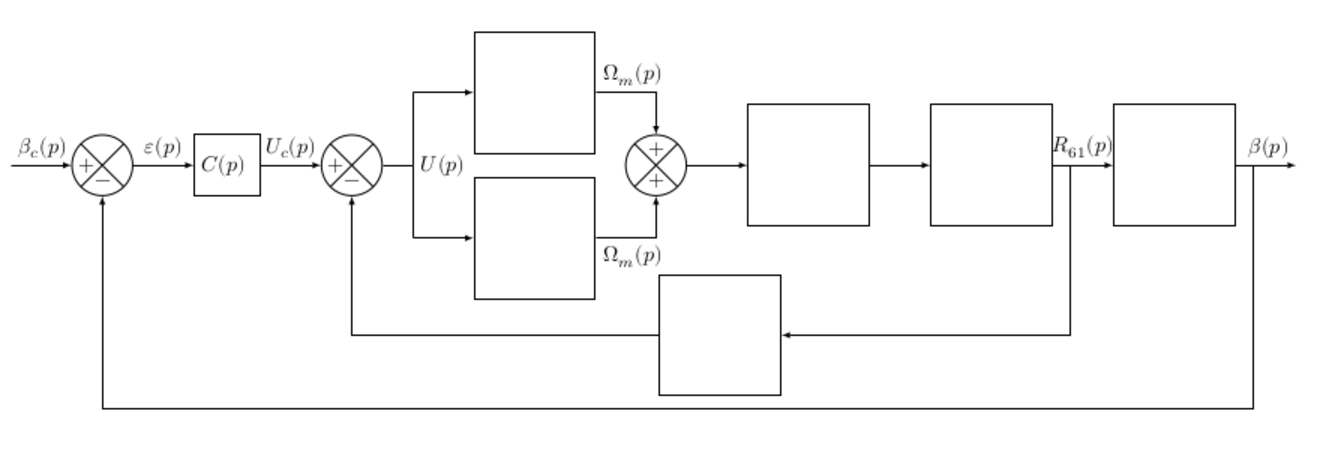
\includegraphics[width=\linewidth]{img/DR2}\end{center}}{\begin{center}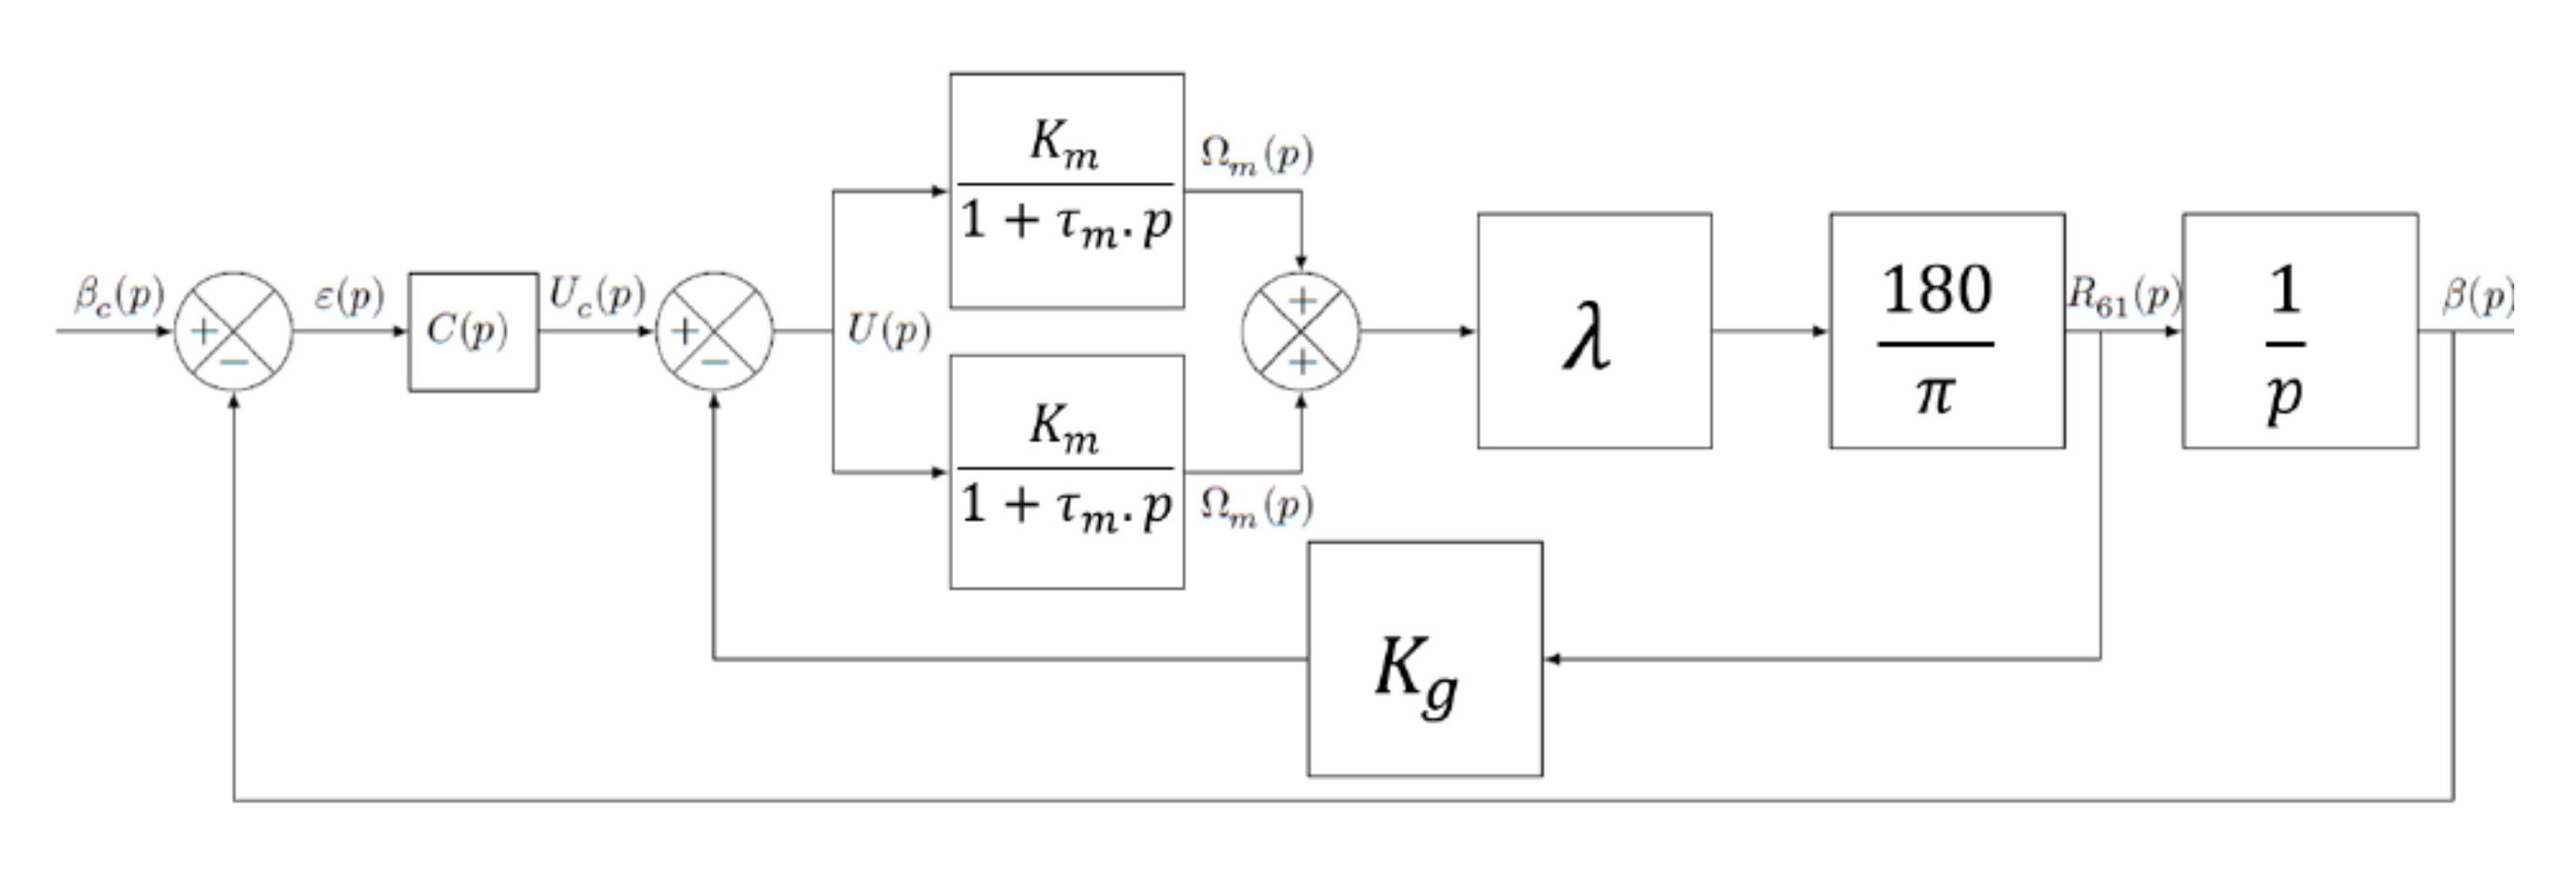
\includegraphics[width=\linewidth]{img/DR2_cor}\end{center}}

\reponse{4}{}{$H(p)=\frac{1}{1+(K_g+\frac{\pi}{360\lambda.K_m})p+\frac{\pi.\tau_m}{360\lambda.K_m}p^2}$}

\newpage

\reponse{1}{\begin{flushright}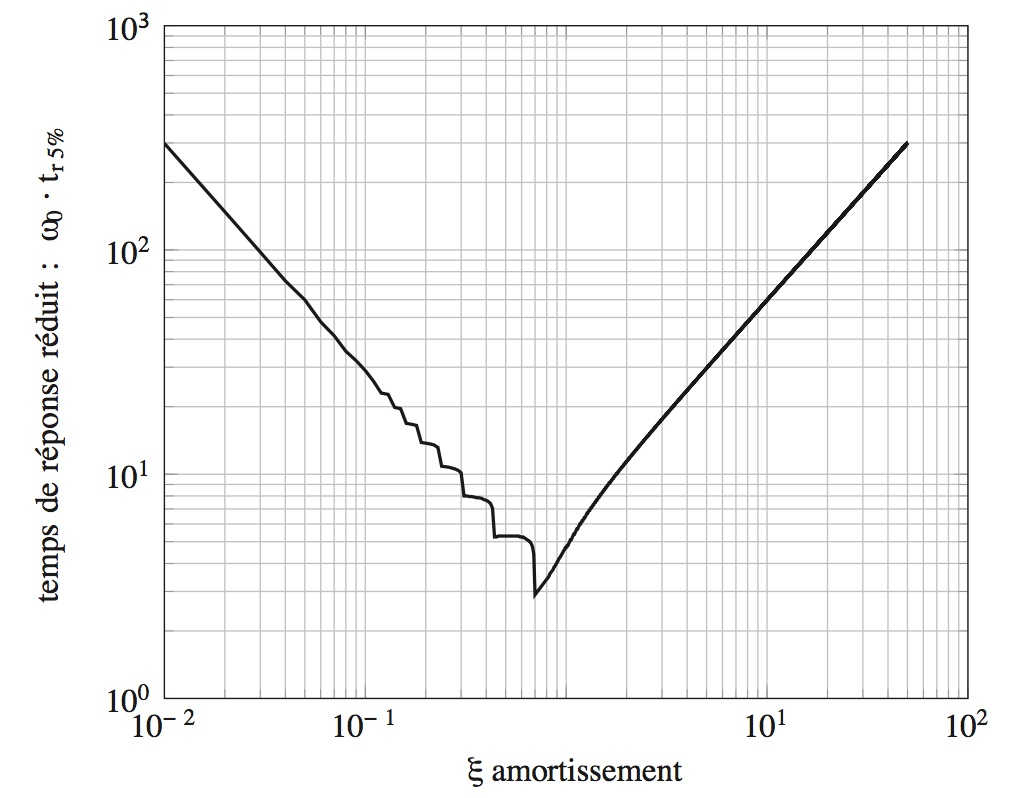
\includegraphics[width=0.6\linewidth]{img/figure_17}\end{flushright}}{\begin{minipage}{0.4\linewidth}$\omega_0=\frac{1}{\sqrt{0,019}}=\sqrt{\frac{100}{1,9}}\approx\frac{10}{\sqrt{2}}$\\
$\omega_0=10\frac{\sqrt{2}}{2}\approx7,1\:rad.s^{-1}$\\
$\xi=\frac{0,17}{\sqrt{0,019}}.\frac{1}{2}=\frac{0,17.7,1}{2}=\frac{1,2}{2}=0,6$\\
$t_{r5\%}.\omega_0=5 $on en déduit $t_{r5\%}=\frac{5}{7,1}\approx0,7s$\end{minipage}\hfill\begin{minipage}{0.55\linewidth}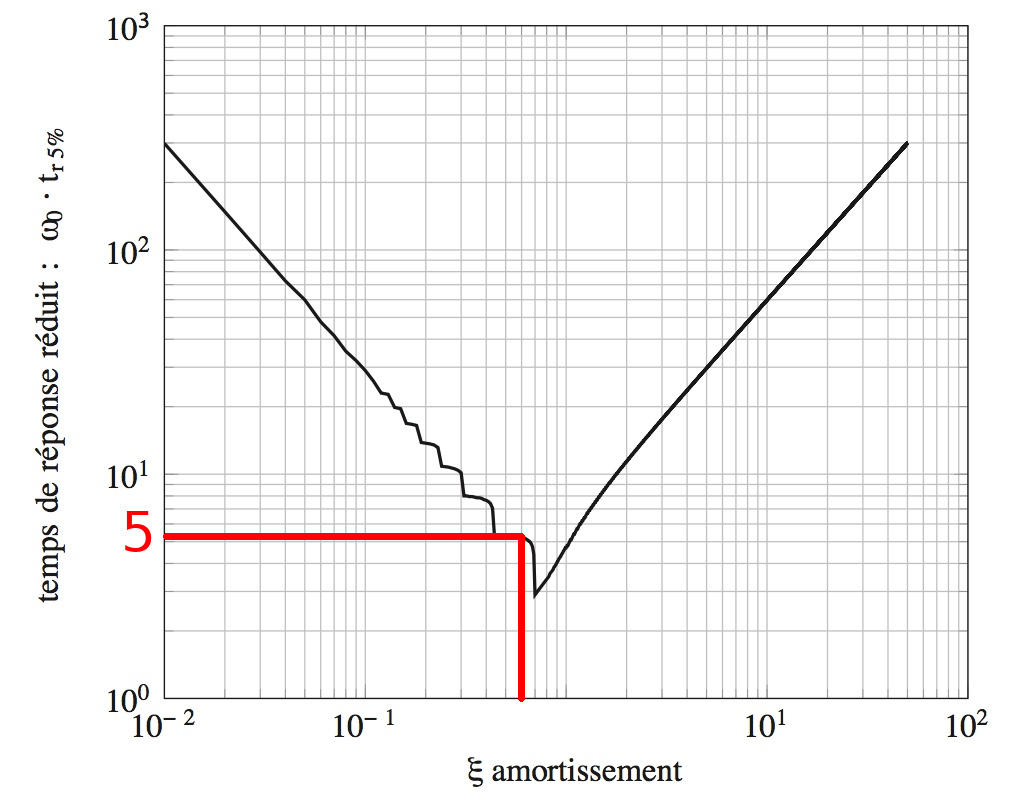
\includegraphics[width=\linewidth]{img/figure_17_cor}\end{minipage}}

\reponse{6}{}{Il y a dépassement, et le temps de réponse est supérieur à 0,3 s donc le cahier des charges n’est pas respecté.}

\reponse{1}{\begin{flushright}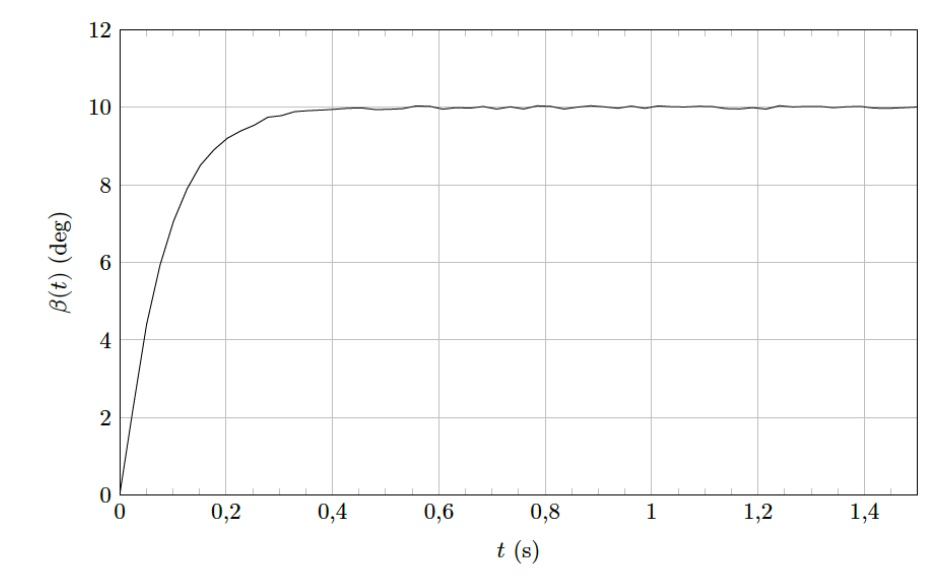
\includegraphics[width=0.7\linewidth]{img/figure_18}\end{flushright}}{\begin{minipage}{0.4\linewidth}
Valeur finale: 10° (pas d’erreur statique)\\
tr5\% = 0,25s < 0,3s

Pas de dépassement

On en déduit que le cahier des charges est maintenant respecté.\end{minipage}\hfill\begin{minipage}{0.55\linewidth}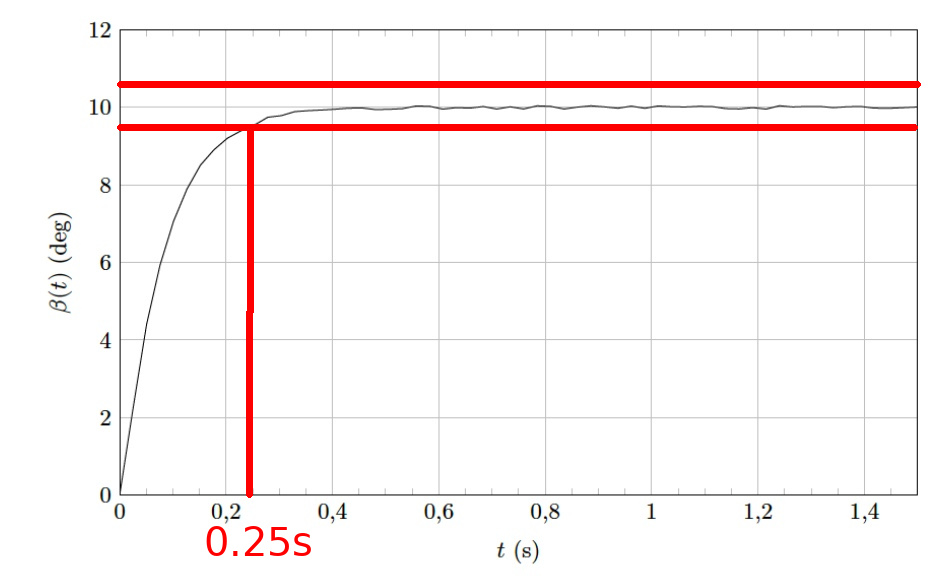
\includegraphics[width=\linewidth]{img/figure_18_cor}\end{minipage}}

\newpage

\reponse{20}{}{Toutes les dimensions au diamètre du cylindre doivent être comprises entre 7,9mm et 8,1mm. Un cylindre parfait de diamètre 7,9mm doit pouvoir rentrer à l'intérieur de la surface réputée cylindrique.}

\reponse{1}{
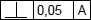
\includegraphics[width=0.15\linewidth]{img/specif1}\\
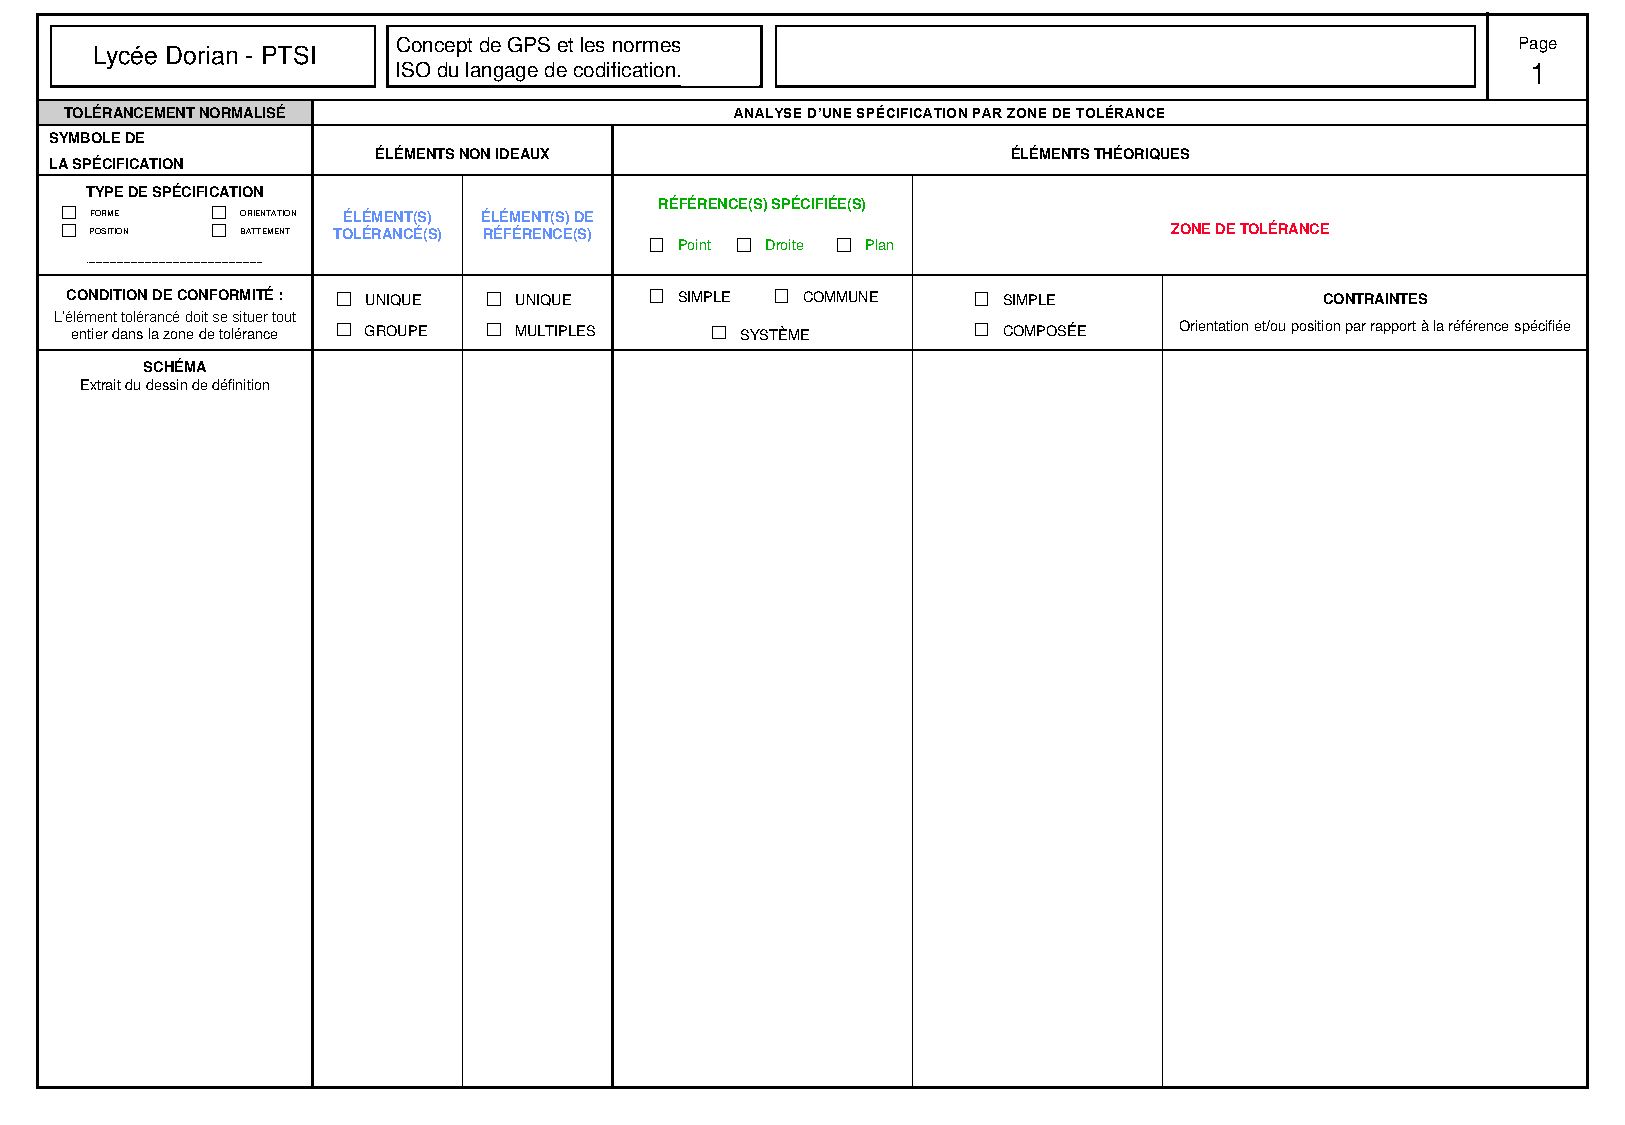
\includegraphics[width=\linewidth]{img/Tableau_GPS_vierge}

\newpage


\includegraphics[width=0.15\linewidth]{img/specif2}\\
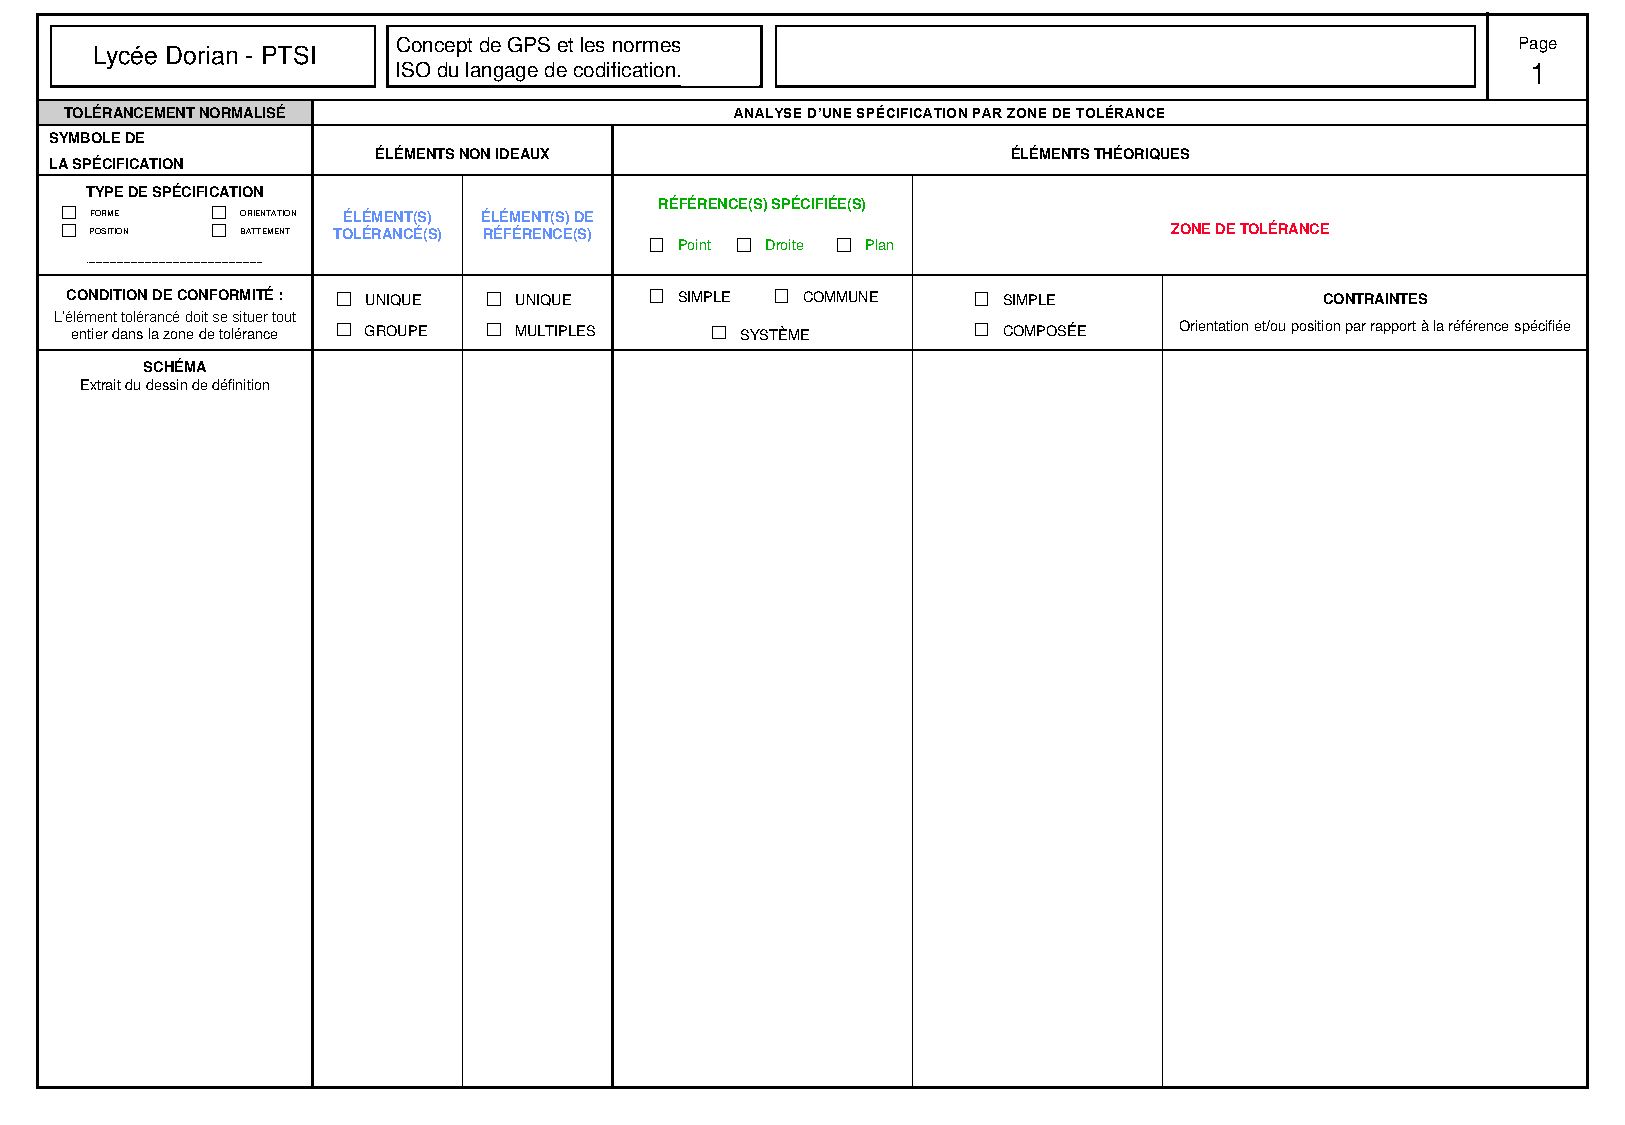
\includegraphics[width=\linewidth]{img/Tableau_GPS_vierge}
}
{
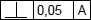
\includegraphics[width=0.15\linewidth]{img/specif1}\\
\textbf{Élément tolérancé:} Surface nominalement plane \\
\textbf{Élément de référence:} Surface nominalement cylindrique \\
\textbf{Référence spécifiée:} Axe du plus petit cylindre circonscrit. \\
\textbf{Zone de tolérance:} Deux plans parallèles distants de 0,05mm perpendiculaires à la référence spécifiée. \\

\includegraphics[width=0.15\linewidth]{img/specif2}\\
\textbf{Élément tolérancé:} Surface nominalement plane \\
\textbf{Élément de référence:} A: Surface nominalement cylindrique \\
B: Surface nominalement plane
\textbf{Référence spécifiée:} A: Axe du plus petit cylindre circonscrit \\
B: Plan perpendiculaire à A, tangent extérieur matière minimisant les écarts maximum.
\textbf{Zone de tolérance:} Deux plans parallèles distants de 0,4mm perpendiculaires à A et dont le plan médian est à 40mm de B.
}

\reponse{10}{}{Le montage à droite est un montage en O car les efforts sont à l'extérieur des roulements. La charge (pignon du montage de gauche) est tournante par rapport à l'arbre, il serait judicieux de serrer les roulements sur l'arbre mais cela n'est pas possible à cause des arrêts axiaux, on suppose qu'il y aura quand même un serrage mais qu'il sera faible. Les arrêt axiaux sont des épaulements sauf sur les extrémités de l'arbre où on trouve une vis/rondelle à gauche et un écrou/rondelle à encoches à droite. Des épaulements sur l'arbre entre les deux roulements permettent de gérer le serrage. Un joint à lèvre est présent à droite, son orientation permet de supposer que la lubrification se fait à l'huile.}

\reponse{10}{}{Le carter n'est pas hachuré car il n'a pas été coupé sur cette vue, il est en deux parties afin de pouvoir enlever le pignon du montage de gauche. Une seule des deux parties est présentée ici.}

\reponse{10}{}{Ici les efforts sont à l'intérieur des roulements, il faut donc mettre en place un montage en X. La charge est toujours tournante par rapport à l'arbre, donc on essayera de serrer les bagues des roulements sur l'arbre.}

\reponse{1}{Cf calque}{}

\reponse{1}{Cf calque}{}

\reponse{1}{Cf calque}{}

\newpage

\ifdef{\public}{\Huge{Calque (échelle 1:1:)}

\begin{center}
	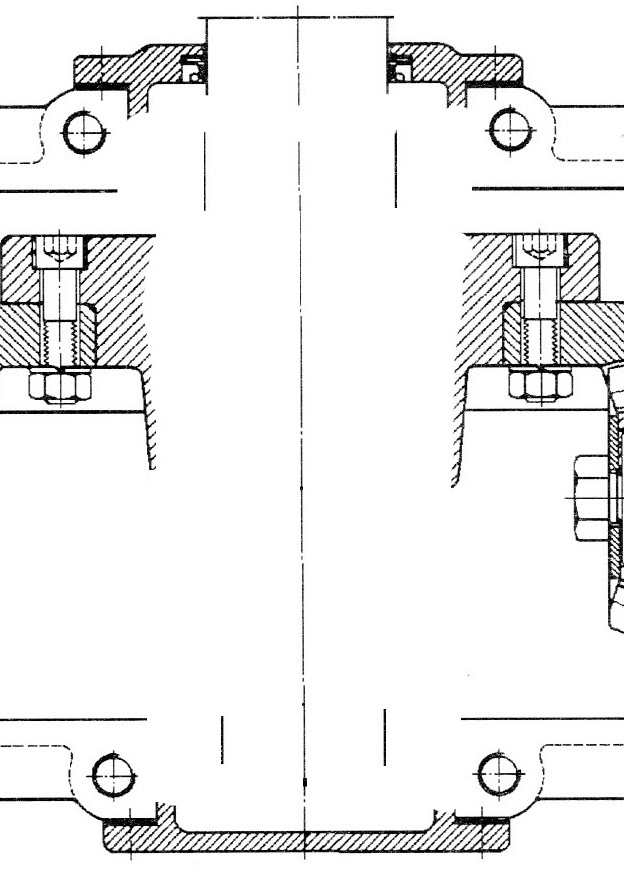
\includegraphics[width=0.9\linewidth]{img/montage_roulements_dr}
\end{center}}{\begin{center}
	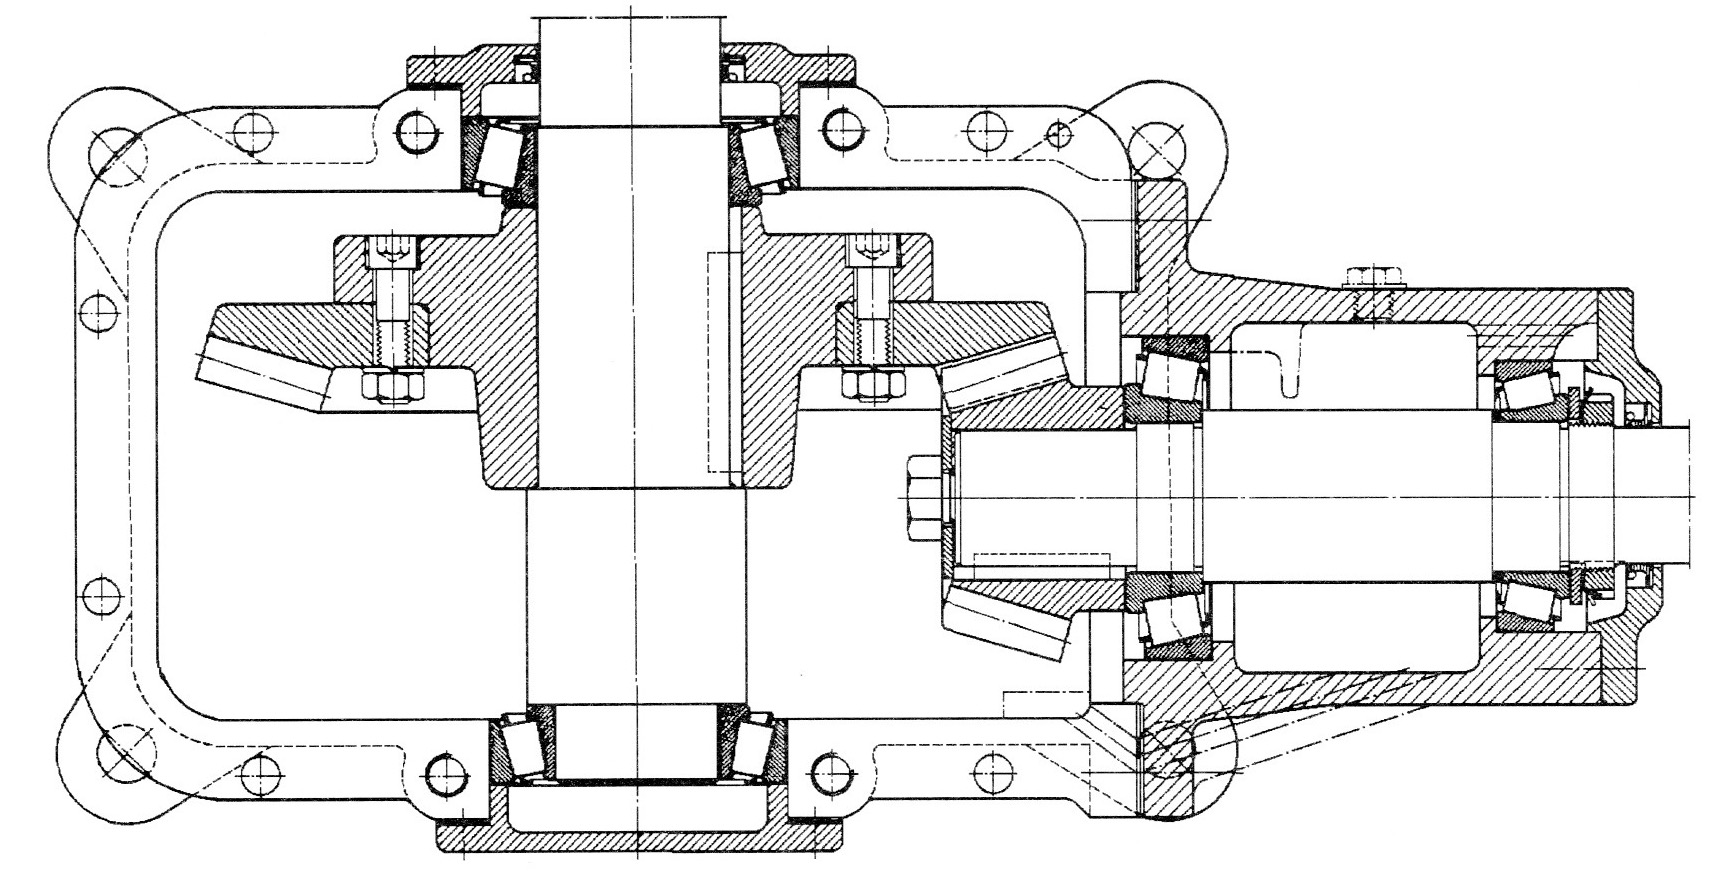
\includegraphics[width=0.9\linewidth]{img/montage_roulements_cor}
\end{center}}



\end{document}